% Modelo UFSC/CTC/DAS para PFCs (08/07/2020)
% Autores: Matheus Bruhns Bastos e Marcelo De Lellis Costa de Oliveira
% --------------------------------------------------------
% Adaptado do arquivo Template-Trabalhos-Academicos-UFSC-A4-v1.3
% disponibilizado em http://portal.bu.ufsc.br/files/2013/10/Template-Trabalhos-Academicos-UFSC-A4-v1.3.zip
% Modelo UFSC para Trabalhos Academicos (tese de doutorado, dissertação de
% mestrado) utilizando a classe abntex2
%
% Autor: Alisson Lopes Furlani
% 	Modificações:
%	- 27/08/2019: Alisson L. Furlani, add 'glossaries' package
%   - 30/10/2019: Alisson L. Furlani, adjusted some spacing errors and changed math fonts
%   - 17/01/2020: Alisson L. Furlani, updated certification page
%   - 07/02/2020: Alisson L. Furlani, fixed table counter bug
%   - 11/03/2020: Alisson L. Furlani, changed greek letters in math and fixed citation style
% ------------------------------------------------------------------------
% ------------------------------------------------------------------------

\documentclass[
	% -- opções da classe memoir --
	12pt,				% tamanho da fonte
	%openright,			% capítulos começam em pág ímpar (insere página vazia caso preciso)
	oneside,			% para impressão no anverso. Oposto a twoside
	a4paper,			% tamanho do papel. 
	% -- opções da classe abntex2 --
	chapter=TITLE,		% títulos de capítulos convertidos em letras maiúsculas
	section=TITLE,		% títulos de seções convertidos em letras maiúsculas
	%subsection=TITLE,	% títulos de subseções convertidos em letras maiúsculas
	%subsubsection=TITLE,% títulos de subsubseções convertidos em letras maiúsculas
	% -- opções do pacote babel --
	brazil,			% idioma adicional para hifenização
	%french,				% idioma adicional para hifenização
	%spanish,			% idioma adicional para hifenização
	english				% o último idioma é o principal do documento
	]{abntex2}

\usepackage{setup/ufscthesisA4-alf}
\addbibresource{aftertext/references.bib} % Seus arquivos de referências

% ---
% Filtering and Mapping Bibliographies
% ---
\DeclareSourcemap{
	\maps[datatype=bibtex]{
		% remove fields that are always useless
		\map{
			\step[fieldset=abstract, null]
			\step[fieldset=pagetotal, null]
		}
		% remove URLs for types that are primarily printed
%		\map{
%			\pernottype{software}
%			\pernottype{online}
%			\pernottype{report}
%			\pernottype{techreport}
%			\pernottype{standard}
%			\pernottype{manual}
%			\pernottype{misc}
%			\step[fieldset=url, null]
%			\step[fieldset=urldate, null]
%		}
		\map{
			\pertype{inproceedings}
			% remove mostly redundant conference information
			\step[fieldset=venue, null]
			\step[fieldset=eventdate, null]
			\step[fieldset=eventtitle, null]
			% do not show ISBN for proceedings
			\step[fieldset=isbn, null]
			% Citavi bug
			\step[fieldset=volume, null]
		}
	}
}
% ---

% ---
% Informações de dados para CAPA e FOLHA DE ROSTO
% ---
\autor{Bruno Machado Pacheco}
% Substituir 'Título do trabalho' pelo título da trabalho.
\titulo{Physics-Informed Deep Equilibrium Models for Solving ODEs}
% Caso não tenha substítulo, comente a linha a seguir.
% \subtitulo{subtitle (if any)}
% Substituir 'XXXXXX' pelo nome do seu
% orientador.
\orientador{Prof. Eduardo Camponogara, Ph.D.}
% Se for orientado por uma mulher, comente a linha acima e descomente a linha a seguir.
% \orientador[Orientadora]{Nome da orientadora, Dra.}
% Substituir 'XXXXXX' pelo nome do seu
% supervisor no local de realização do PFC. Caso não tenha supervisor, comente a linha a seguir.
% \coorientador{YYYYY, Eng.}
% Se for supervisionado por uma mulher, comente a linha acima e descomente a linha a seguir.
% \coorientador[Supervisora]{XXXXXX, Eng.}
% Substituir '[ano]' pelo ano (ano) em que seu trabalho foi defendido.
\ano{2022}
% FIXME Substituir '[dia] de [mês] de [ano]' pela data em que ocorreu sua defesa.
%\data{[dia] de [mês] de [ano]}
% Substituir 'Local' pela cidade em que ocorreu sua defesa.
\local{Florianópolis}
\instituicaosigla{UFSC}
\instituicao{Federal University of Santa Catarina}
% Substituir 'Dissertação/Tese' pelo tipo de trabalho (Tese, Dissertação). 
\tipotrabalho{Final report of the subject DAS5511 (Course Final Project) as a Concluding Dissertation}
%Relatório final da disciplina DAS5511 (Projeto de Fim de Curso) como Trabalho de Conclusão}
\formacao{Control and Automation Engineer}
% Substituir '[mestrado/doutorado]' pelo nivel adequado.
\nivel{[mestrado/doutorado]}
% Substituir 'Programa de Pós-Graduação em XXXXXX' pela curso adequado.
\programa{Programa de Pós-Graduação em XXXXXX}
\centro{Technology Center}
\departamento{Department of Automation and Systems Engineering}
\curso{Undergraduate Program in Control and Automation Engineering}
\preambulo
{%
%\imprimirtipotrabalho~do~\imprimircurso~da~\imprimirinstituicao~como~requisito~para~a~obtenção~do~título~de~\imprimirformacao.
\imprimirtipotrabalho~of the~\imprimircurso~of the~\imprimirinstituicao.
}
% ---

% ---
% Configurações de aparência do PDF final
% ---
% alterando o aspecto da cor azul
\definecolor{blue}{RGB}{41,5,195}
% informações do PDF
\makeatletter
\hypersetup{
     	%pagebackref=true,
		pdftitle={\@title}, 
		pdfauthor={\@author},
    	pdfsubject={\imprimirpreambulo},
	    pdfcreator={LaTeX with abnTeX2},
		pdfkeywords={ufsc, latex, abntex2}, 
		colorlinks=true,       		% false: boxed links; true: colored links
    	linkcolor=black,%blue,          	% color of internal links
    	citecolor=black,%blue,        		% color of links to bibliography
    	filecolor=black,%magenta,      		% color of file links
		urlcolor=black,%blue,
		bookmarksdepth=4
}
\makeatother
% ---

% ---
% compila a lista de abreviaturas e siglas e a lista de símbolos
% ---

% Declaração das siglas
\siglalista{ABNT}{Associação Brasileira de Normas Técnicas}
\siglalista{ODE}{ordinary differential equation}
\siglalista{PINN}{physics-informed neural network}
\siglalista{DEQ}{deep equilibrium model}
\siglalista{PIDEQ}{physics-informed deep equilibrium model}
\siglalista{IVP}{initial-value problem}
\siglalista{RK4}{classic Runge-Kutta method}
\siglalista{IAE}{integral of absolute error}

% Declaração dos simbolos
\simbololista{lr}{\ensuremath{\gamma}}{Learning rate}
\simbololista{param}{\ensuremath{\theta}}{Parameter vector}
\simbololista{sigmoid}{\ensuremath{\sigma}}{Sigmoid function}
% \simbololista{r}{\ensuremath{r}}{Raio de um círculo}
% \simbololista{A}{\ensuremath{A}}{Área de um círculo}

% compila a lista de abreviaturas e siglas e a lista de símbolos
\makenoidxglossaries 

% ---

% ---
% compila o indice
% ---
\makeindex
% ---

% ----
% Início do documento
% ----
\begin{document}

% Seleciona o idioma do documento (conforme pacotes do babel)
\selectlanguage{english}

% Retira espaço extra obsoleto entre as frases.
\frenchspacing 

% Espaçamento 1.5 entre linhas
\OnehalfSpacing

% Corrige justificação
%\sloppy

% ----------------------------------------------------------
% ELEMENTOS PRÉ-TEXTUAIS
% ----------------------------------------------------------
% \pretextual %a macro \pretextual é acionado automaticamente no início de \begin{document}
% ---
% Capa, folha de rosto, ficha bibliografica, errata, folha de apróvação
% Dedicatória, agradecimentos, epígrafe, resumos, listas
% ---
% ---
% Capa
% ---
\imprimircapa
% ---

% ---
% Folha de rosto
% (o * indica que haverá a ficha bibliográfica)
% ---
\imprimirfolhaderosto*
% ---

% ---
% Inserir a ficha bibliografica
% ---
% http://ficha.bu.ufsc.br/
\begin{fichacatalografica}
	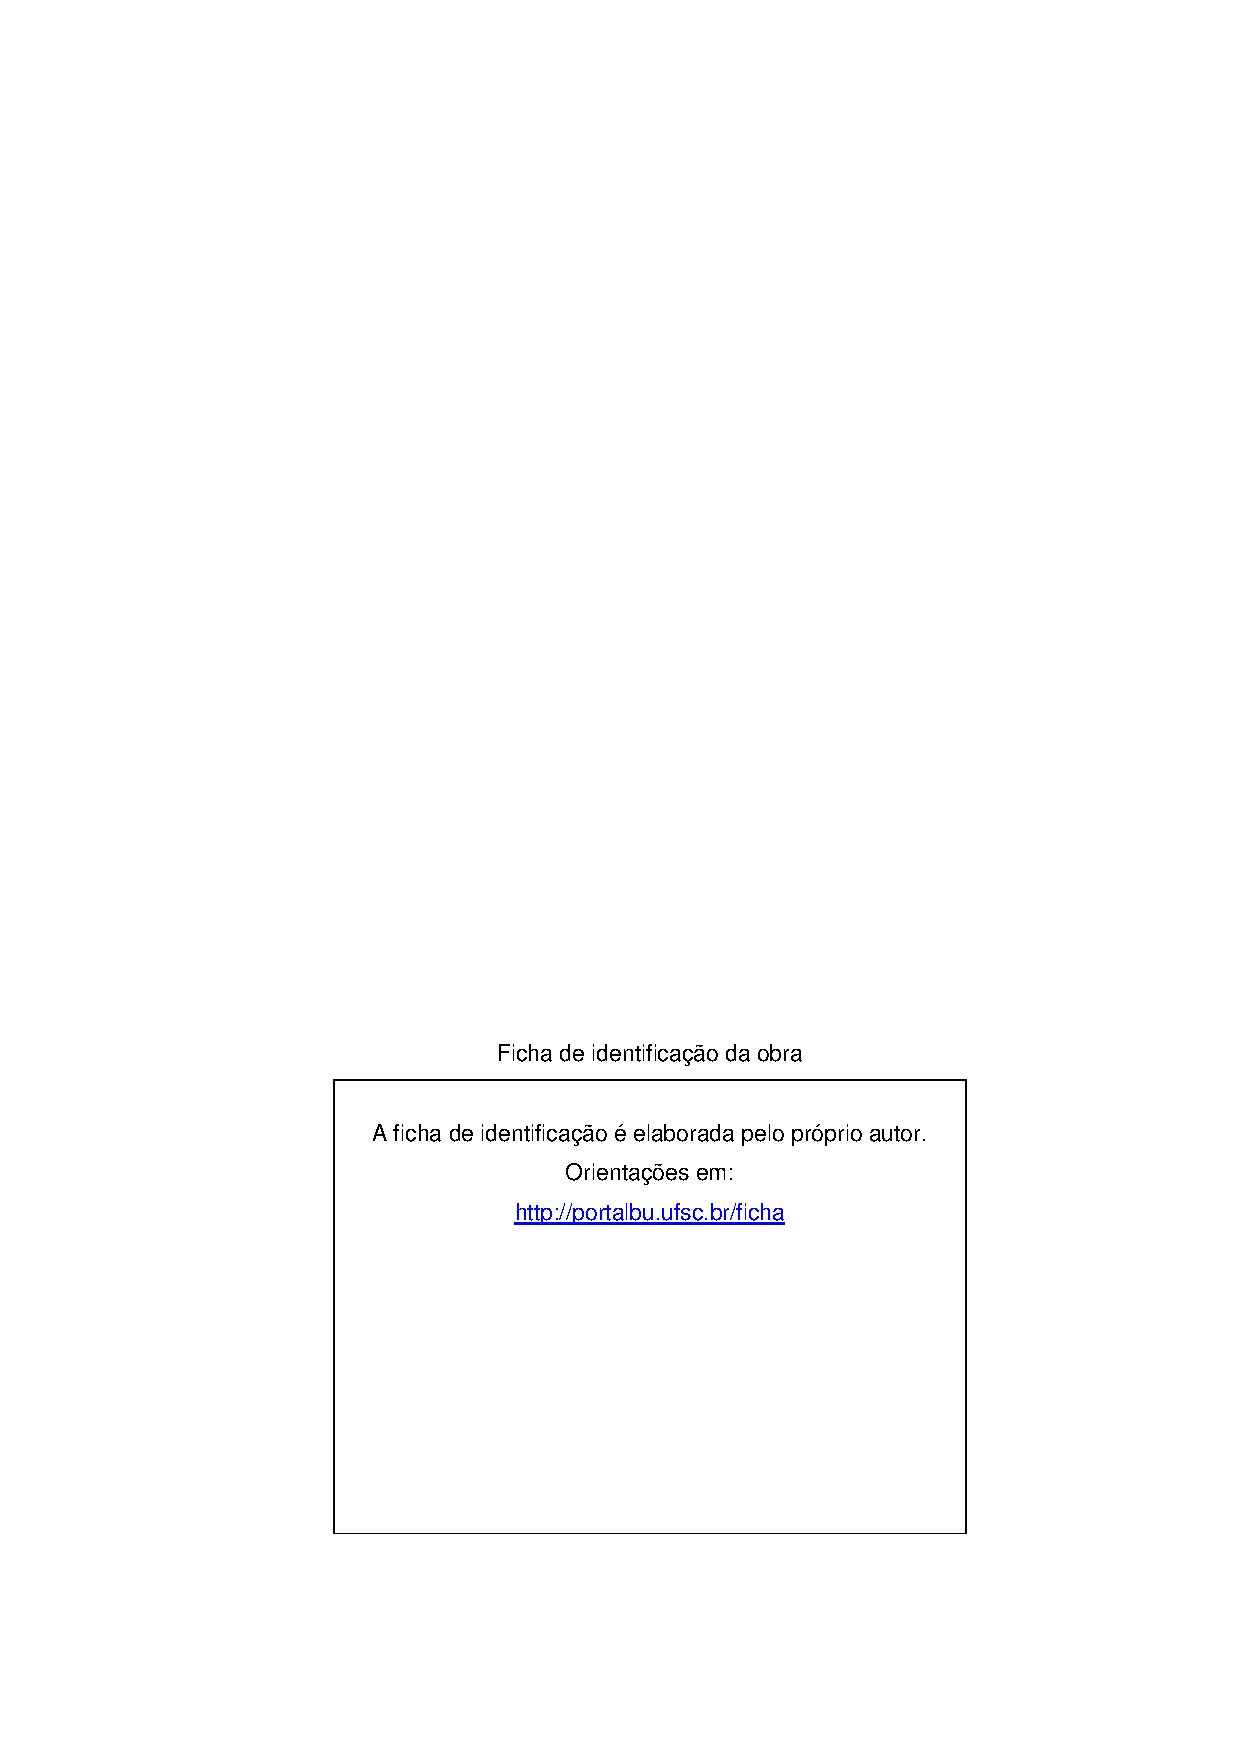
\includepdf{beforetext/Ficha_Catalografica.pdf}
\end{fichacatalografica}
% ---

% ---
% Inserir folha de aprovação
% ---
\begin{folhadeaprovacao}
	\OnehalfSpacing
	\centering
	\imprimirautor\\%
	\vspace*{10pt}		
	\textbf{\imprimirtitulo}%
	\ifnotempty{\imprimirsubtitulo}{:~\imprimirsubtitulo}\\%
	%		\vspace*{31.5pt}%3\baselineskip
	\vspace*{\baselineskip}
	
	This dissertation was evaluated in the context of the subject DAS5511 (Course Final Project) and approved in its final form by the \imprimircurso\\
	%Esta monografia foi julgada no contexto da disciplina DAS5511 (Projeto de Fim de Curso) e aprovada em sua forma final pelo \imprimircurso\\
	\vspace*{\baselineskip}
	Florianópolis, <month> <day>, <year>.\\
	
	%%%%%%%%%%%%%%%%%%%%%%%%%%%%%%%%%%%%%%%%%%%%%
	%IMPORTANT: no signatures are required below!
	%%%%%%%%%%%%%%%%%%%%%%%%%%%%%%%%%%%%%%%%%%%%%
	
	\vspace*{2\baselineskip}
	%\rule{0.4\textwidth}{0.4pt}\\
	Prof. xxxx, Dr.\\
	Course Coordinator\\
	
	\vspace*{\baselineskip}
	\textbf{Examining Board:} \\
	
	
	\vspace*{2\baselineskip}
	%\rule{0.4\textwidth}{0.4pt}\\
	Prof. xxxx, Dr.\\
	Advisor \\
	UFSC/CTC/DAS\\
	
	\vspace*{2\baselineskip}
	%\rule{0.4\textwidth}{0.4pt}\\
	xxxx, Eng.\\
	Supervisor \\
	Company/University xxxx\\
	
	\vspace*{2\baselineskip}
	%\rule{0.4\textwidth}{0.4pt}\\
	Prof. xxxx, Dr.\\
	Evaluator \\
	Instituição xxxx\\
	
	\vspace*{2\baselineskip}
	%\rule{0.4\textwidth}{0.4pt}\\
	Prof. xxxx, Dr.\\
	Board President \\
	UFSC/CTC/DAS
\end{folhadeaprovacao}
% ---

% ---
% Dedicatória
% ---
\begin{dedicatoria}
	\vspace*{\fill}
	\noindent
	\begin{adjustwidth*}{}{5.5cm} 
		\raggedleft       
		This work is dedicated to my classmates and my dear parents.
	\end{adjustwidth*}
\end{dedicatoria}
% ---

% ---
% Agradecimentos
% ---
\begin{agradecimentos}
	Inserir os agradecimentos aos colaboradores à execução do trabalho. 
	
	Xxxxxxxxxxxxxxxxxxxxxxxxxxxxxxxxxxxxxxxxxxxxxxxxxxxxxxxxxxxxxxxxxxxxxx. 
\end{agradecimentos}
% ---

% ---
% Epígrafe
% ---
\begin{epigrafe}
	\vspace*{\fill}
	\begin{flushright}
		\textit{``Texto da Epígrafe.\\
			Citação relativa ao tema do trabalho.\\
			É opcional. A epígrafe pode também aparecer\\
			na abertura de cada seção ou capítulo.\\
			Deve ser elaborada de acordo com a NBR 10520.''\\
			(SOBRENOME do autor da epígrafe, ano)}
	\end{flushright}
\end{epigrafe}
% ---

% ---
% RESUMOS
% ---

% resumo em português
\setlength{\absparsep}{18pt} % ajusta o espaçamento dos parágrafos do resumo
\begin{resumo}
	\SingleSpacing
	\textbf{Instruções do padrão genérico de TCCs da BU:}
	No resumo são ressaltados o objetivo da pesquisa, o método utilizado, as discussões e os resultados com destaque apenas para os pontos principais. O resumo deve ser significativo, composto de uma sequência de frases concisas, afirmativas, e não de uma enumeração de tópicos. Não deve conter citações. Deve usar o verbo na voz ativa e na terceira pessoa do singular. O texto do resumo deve ser digitado, em um único bloco, sem espaço de parágrafo. O espaçamento entre linhas é simples e o tamanho da fonte é 12. Abaixo do resumo, informar as palavras-chave (palavras ou expressões significativas retiradas do texto) ou, termos retirados de thesaurus da área. Deve conter de 150 a 500 palavras. O resumo é elaborado de acordo com a NBR 6028. \textbf{Instruções da Coordenação do PFC:} o resumo deve contextualizar o trabalho e descrever de forma sucinta o problema, a solução proposta, a metodologia utilizada e os resultados obtidos. Tudo de forma bem resumida e direta, sem entrar em detalhes técnicos.
	
	\textbf{Keywords}: Keyword 1. Keyword 2. Keyword 3.
\end{resumo}

% resumo em inglês
\begin{resumo}[Resumo]
	\SingleSpacing
	\begin{otherlanguage*}{brazil}
		Resumo traduzido para outros idiomas, neste caso, português. Segue o formato do resumo feito na língua vernácula. As palavras-chave traduzidas, versão em língua estrangeira, são colocadas abaixo do texto precedidas pela expressão “Keywords”, separadas por ponto.
		
		\textbf{Palavras-chave}: Palavra-chave 1. Palavra-chave 2. Palavra-chave 3.
	\end{otherlanguage*}
\end{resumo}

%% resumo em francês 
%\begin{resumo}[Résumé]
% \begin{otherlanguage*}{french}
%    Il s'agit d'un résumé en français.
% 
%   \textbf{Mots-clés}: latex. abntex. publication de textes.
% \end{otherlanguage*}
%\end{resumo}
%
%% resumo em espanhol
%\begin{resumo}[Resumen]
% \begin{otherlanguage*}{spanish}
%   Este es el resumen en español.
%  
%   \textbf{Palabras clave}: latex. abntex. publicación de textos.
% \end{otherlanguage*}
%\end{resumo}
%% ---

{%hidelinks
	\hypersetup{hidelinks}
	% ---
	% inserir lista de ilustrações
	% ---
	\pdfbookmark[0]{\listfigurename}{lof}
	\listoffigures*
	\cleardoublepage
	% ---
	
	% ---
	% inserir lista de quadros
	% ---
	\pdfbookmark[0]{\listofquadrosname}{loq}
	\listofquadros*
	\cleardoublepage
	% ---
	
	% ---
	% inserir lista de tabelas
	% ---
	\pdfbookmark[0]{\listtablename}{lot}
	\listoftables*
	\cleardoublepage
	% ---
	
	% ---
	% inserir lista de abreviaturas e siglas (devem ser declarados no preambulo)
	% ---
	\imprimirlistadesiglas
	% ---
	
	% ---
	% inserir lista de símbolos (devem ser declarados no preambulo)
	% ---
	\imprimirlistadesimbolos
	% ---
	
	% ---
	% inserir o sumario
	% ---
	\pdfbookmark[0]{\contentsname}{toc}
	\tableofcontents*
	\cleardoublepage
	
}%hidelinks
% ---
% ---

% ----------------------------------------------------------
% ELEMENTOS TEXTUAIS
% ----------------------------------------------------------
\textual

% ---
% 1 - Introdução
% ---
% ----------------------------------------------------------
\chapter{Introdução}
% ----------------------------------------------------------

\textbf{Instruções do padrão genérico de TCCs da BU:}

As orientações aqui apresentadas são baseadas em um conjunto de normas elaboradas pela \gls{ABNT}. Além das normas técnicas, a Biblioteca também elaborou uma série de tutoriais, guias, \textit{templates} os quais estão disponíveis em seu site, no endereço \url{http://portal.bu.ufsc.br/normalizacao/}.

Paralelamente ao uso deste \textit{template} recomenda-se que seja utilizado o \textbf{Tutorial de Trabalhos Acadêmicos} (disponível neste link \url{https://repositorio.ufsc.br/handle/123456789/180829}).

Este \textit{template} está configurado apenas para a impressão utilizando o anverso das folhas, caso você queira imprimir usando a frente e o verso, acrescente a opção \textit{openright} e mude de \textit{oneside} para \textit{twoside} nas configurações da classe \textit{abntex2} no início do arquivo principal \textit{main.tex} \cite{abntex2classe}.

Conforme a \href{https://repositorio.ufsc.br/bitstream/handle/123456789/197121/RN46.2019.pdf?sequence=1&isAllowed=y}{Resolução NORMATIVA nº 46/2019/CPG} as dissertações e teses não serão mais entregues em formato impresso na Biblioteca Universitária. Consulte o Repositório Institucional da UFSC ou sua Secretaria de Pós Graduação sobre os procedimentos para a entrega. 

\nocite{NBR6023:2002}
\nocite{NBR6027:2012}
\nocite{NBR6028:2003}
\nocite{NBR10520:2002}

\textbf{Instruções da Coordenação do PFC:}

Neste primeiro capítulo é muito importante deixar bem claro (de uma maneira mais resumida, sem entrar em detalhes técnicos, apenas para passar a ideia geral ao leitor):

\begin{itemize}
    \item o problema tratado no PFC;
    \item a importância do problema para a empresa ou instituição em que o PFC foi realizado;
    \item a solução proposta;
    \item a metodologia utilizada;
    \item os resultados obtidos e a sua importância para a empresa/clientes;
    \item o que de fato foi feito pelo autor, diferenciando do que foi aproveitado de trabalhos anteriores/outras equipes da empresa. \textbf{Importante}: esta preocupação em diferenciar o trabalho do autor daquele de possíveis colegas em um trabalho em equipe deve permear todo o documento.
\end{itemize}

Apesar de o tamanho da monografia não ter uma correlação direta com a nota, bons trabalhos não costumam ser relatados suficientemente bem com menos de 50 páginas. Acima de 100 páginas a monografia pode se tornar ``massante'', discorrendo além do necessário para o entendimento do trabalho, portanto perdendo o foco do leitor.

A linguagem a ser utilizada em um trabalho acadêmico deve ser técnico-científica, portanto formal (e não informal, como se o trabalho estivesse sendo explicado a um colega ou familiar). Portanto não devem ser usadas gírias. Utilize correto ortográfico e verifique a gramática (pontuação, uso da vírgula, concordância, coesão textual etc.).

% ----------------------------------------------------------
\section{Objetivos}
% ----------------------------------------------------------

Aqui são descritos os objetivos, que podem ser estratificados em objetivo geral e objetivos específicos.

Outra opção é colocar os objetivos específicos na forma de passos de uma metodologia de trabalho, ou seja, os procedimentos e ferramentas adotadas em cada fase do projeto (um plano de trabalho).

\section*{Estrutura do documento}

Ao final do capítulo introdutório, costuma-se descrever como o documento está estruturado (encadeamento dos próximos capítulos). A estruturação sugerida a seguir é em linhas gerais e não precisa ser seguida à risca: dependendo da área e foco do trabalho, o número de capítulos pode variar. O estudante deve consultar seu orientador na UFSC para definir a estrutura do documento.

No capítulo \ref{cap:desenvolvimento} é feita uma descrição da empresa (instituição de realização do PFC) e seus processos/produtos.

No capítulo 3 é apresentada uma fundamentação teórica: são discutidas teorias, modelos etc. fundamentais para o entendimento da solução proposta.

No capítulo 4 são expostos os requisitos gerais, funcionais e não-funcionais, a serem considerados no projeto. Também podem ser utilizados fluxos de informação e materiais, diagramas etc., para delinear os resultados que a solução proposta deve atingir. Aqui pode ser elaborado um modelo da planta acompanhado de identificação, por exemplo.

No capítulo 5 é descrito em detalhes o projeto (\emph{hardware}, \emph{software}) feito. Para isto a solução é formalizada por meio de diagramas, casos de uso, interfaces gráficas, projeto de controladores. as decisões que foram tomadas e o seu porquê, em alinhamento com os requisitos colocados. Na área de controle, aqui pode ser feito o projeto do controlador.

No capítulo 6 é feita uma análise de resultados: vantagens e desvantagens, impactos dos resultados nos processos da empresa. Para isto devem ser utilizados indicadores, gráficos, estatísticas etc.

No último capítulo é feita uma conclusão do PFC. Ela compreende um resumo do que foi feito, retomando a motivação do trabalho, a solução proposta e os principais resultados atingidos. Também deve ser feita uma análise das limitações do projeto, e apontadas possíveis melhorias caso o trabalho venha a ser continuado (sugestão de trabalhos futuros).
% ---

% ---
% 2 - ODEs
% ---
% ----------------------------------------------------------
\chapter{Ordinary Differential Equations}
% ----------------------------------------------------------

This first chapter is a short review of \gls{ODE}s and how to solve them numerically.
It would be unreasonable to assume that one chapter of a bachelor thesis could cover what many authors have dedicated entire books to communicate.
Therefore, it is assumed that the reader has a basic (undergraduate level) understanding of the theory of differential equations\footnotemark.
\footnotetext{Otherwise, the books of \textcite{zill_first_2013} and \textcite{simmons_differential_2017} are great resources.}
This way, this chapter focuses on reviewing the fundamentals and establishing a notation concise for the following chapters, besides introducing the approach to numerical solve \gls{ODE}s.

\section{Introduction and Definitions}

A differential equation can be seen as a description of the relationship between unknown quantities and their rates of changes.
Because of this broader definition and direct relationship to applications, differential equations arise naturally in many fields of applied sciences\cite{hairer_solving_1993}, as it is often the case that the rate of change of a certain quantity of interest is related to the rate of change of other quantities.
A classical example of a differential equation is Newton's second law of motion \[
F\left( x\left( t \right) \right) = m \frac{d^2 y(t)}{d t^2}
,\] in which $x\left( t \right) $ is the position of an object at time $t$, $m$ is its mass, and $F(x)$ is the force under which the object is at a given position.
This example highlights one of the great powers of the differential equations, which is to describe the dynamics of a certain phenomenon without explicitly defining it.


For a more tangible definition, any equation that contains the derivatives of (at least) one unknown function with respect to (at least) one independent variable is called a \emph{differential equation}\cite{zill_first_2013}.
A differential equation that involves only \emph{ordinary} derivatives, that is, only derivatives of functions with respect to a single variable, (such as the one above) is called an \gls{ODE}.
% A differential equation can also be classified through its \emph{order} (the order of its highest derivative)
\gls{ODE}s can be represented in the normal form
\begin{equation}\label{eq:ode}
    \frac{d^n \bm{y}(t)}{d t^{n}} = \mathcal{N}\left( t, \bm{y}\left( t \right), \frac{d \bm{y}(t)}{d t}, \ldots,\frac{d^{n-1}\bm{y}(t)}{d t^{n-1}} \right)
\end{equation}
%\gls{ODE}s can be represented in the normal form \[
    %\frac{d^n \bm{y}(t)}{d t^{n}} = \mathcal{N}\left( t, \bm{y}\left( t \right), \frac{d \bm{y}(t)}{d t}, \ldots,\frac{d^{n-1}\bm{y}(t)}{d t^{n-1}} \right) \tag{$*$}\label{eq:ode}
in which $\bm{y}\left( t \right) $ is a vector-valued continuous function, $\mathcal{N}:\R\times \R^{n}\to \R$ is a real-valued continuous function, and $n$ is the order of the highest derivative in the equation and is commonly referred to as the \emph{order of the differential equation}.

\section{Initial Value Problems}

It is a common problem to find an explicit definition of the unknown functions in a differential equation.
Given an $n$-th order ODE such as \eqref{eq:ode}, any function $\bm{\phi}:I\subset\R\to \R^{m}$ is said to be a \emph{solution} of this equation if it satisfies \[
    \frac{d^n \bm{\phi}(t)}{d t^{n}} = \mathcal{N}\left( t, \bm{\phi}\left( t \right) , \frac{d \bm{\phi}(t)}{d t}, \ldots,\frac{d^{n-1}\bm{\phi}(t)}{d t^{n-1}} \right),\,\forall t\in I
.\] Note, however, that the solutions are not necessarily unique.
As an example, given Newton's second law of motion with constant force ($F(x)=C$), then it is easy to see that any second-order polynomial of the form \[
    \phi\left( t \right) = \frac{C}{2m}t^2 + a_1t + a_0,\, a_0,a_1\in \R
\] is a solution.

Yet, for ODEs, it is often the case that if one has $n$ side conditions on the (lowest order) derivatives of the unknown function, than the solution exists and is unique. More precisely, for an ODE defined as in \eqref{eq:ode}, conditions of the form \[
\bm{y}\left( t_0 \right) =\bm{y}_0,\frac{d\bm{y}\left( t_1 \right) }{dt_1}=\bm{y}_1,\ldots,\frac{d^{n-1}\bm{y}\left( t_{n-1} \right) }{dt^{n-1}}= \bm{y}_{n-1}
,\] in which $t_0,\ldots,t_{n-1}\in I\subset \R$ and $y_0,\ldots,y_{n-1}\in R\subset \R^m$, $R$ a rectangle, guarantee the existence and uniqueness of the solution in $I$ if $\mathcal{N}$ is an analytic function\footnotemark in $I\times R$, which is the case for many practical applications.
\footnotetext{A function is said analytic if and only if its Taylor series expansion converges in the entirety of its domain.[REFTO Iserles, 2008]}
The problem of finding the solution given conditions as above is called the \gls{IVP}.

\gls{IVP} shows up frequently when the current (or past) state of a system is known and the future state is desired.
Recalling Newton's second law example, suppose that, besides $F(x)=C$, it is also known that the object lies still at $t=0$, i.e., \[
y(0) = 0,\,\frac{d y(0)}{dt}=0
,\] and we are interested in the solution in the interval $I=\left[ 0,T \right] $, for $T>0$. Then, the only solution is that with $a_0=a_1=0$, that is, \[
    \phi\left( t \right) = \frac{C}{2m}t^2
.\] 

\section{Numerical Solvers}

\section{Van der Pol Oscillator}


% ---

% ---
% 3 - Deep Learning
% ---
% ----------------------------------------------------------
\chapter{Deep Learning}\label{ch:deep-learning}
% ----------------------------------------------------------

In this chapter, a brief overview of the key elements of deep learning are presented.
Deep Learning is a broad area of knowledge that can be seen (and presented) through many viewpoints, which results in a multitude of notations and few well-established naming conventions.
Here, the approach of \textcite{goodfellow_deep_2016} is followed, being altered only to make it consistent with the other chapters.
Furthermore, even though physics-informed learning and implicit models can be seen as branches of deep learning, they are introduced in separated chapters for their relevance.

% ----------------------------------------------------------
\section{Origin/Introduction/Definition?}
% ----------------------------------------------------------

Even though \textit{Deep Learning} may seem like a novel and exciting technology, it has been studied under many different names since the 1940s \cite{goodfellow_deep_2016}.
Deep learning involves composing multiple levels\footnote{The understanding of these levels as a learning \textit{depth} is the origin of the naming for deep learning.} of representation learning.
Representation learning, in turn, is about automatically extracting higher level features from the input data \cite{lecun_deep_2015,bengio_representation_2013}, aiming to facilitate the extraction of useful information, for example, to classify the data into given categories.

Following these definitions, we can see a deep learning \textit{model} as a function with multiple levels of representations.
A simple way of putting this definition into terms would be to define a model with $L$ \emph{layers} of representations as a function $D$ such that, for a given input $x$,
\begin{equation}\label{eq:dl-model}
\begin{split}
    z^{[0]} &= x \\
    z^{[i]} &= f^{[i]}(z^{[i-1]}),\,i=1,\ldots,L \\
    D(x) &= z^{[L]}.
\end{split}
\end{equation}
From this notation, it is easy to see that each function $f^{[i]}$ maps the outputs of the previous layer into the input of the next, ideally achieving a higher abstraction level.

In this context, we can see the goal of \textit{learning} as finding parameters $\gls{param}$ such that the layers indeed extract the desired information, culminating in the model returning the desired output.
A classic toy example in deep learning models is to approximate the Exclusive-OR function, that is, to find a model $D : \R^2 \to \R$ such that
\begin{align*}
    D([0,0]^T) = D([1,1]^T) = 0 \\
    D([1,0]^T) = D([0,1]^T) = 1 \\
.\end{align*}
We can construct this model's layers as functions $f^{[1]}:\R^2\to\R^2$ and $f^{[2]}:\R^2\to\R$ such that
\begin{align*}
    f^{[1]}(\bm{z}) &= \begin{bmatrix}
    OR(\bm{z}) \\
    NAND(\bm{z})
    \end{bmatrix} \\
    f^{[2]}(\bm{z}) &= AND(\bm{z})
.\end{align*}
Note how these functions are extracting simple information from the input, yet their stacking can approximate very well the desired behavior.

\section{Deep Feedforward Networks}\label{sec:neural-nets}

Deep feedforward networks, often times also called \emph{Neural Networks}\footnotemark, are the most essential deep learning models.
\footnotetext{Neural Networks are usually regarded as a more broad set of models, that include the deep feedforward networks. However, for the sake of simplicity, both will be treated as synonyms in this work.}
They were inspired by the works of \textcite{rosenblatt_perceptron_1957} and refined through the many decades since, culminating in one of the most important deep learning models for practitioners and the basis of the most prominent results seen in the recent years \cite{goodfellow_deep_2016}.

In this model, each component is a simple affine operator followed by a nonlinear \textit{activation} function, i.e., following the notation previously presented, we can define a deep feedforward neural network $D_{\gls{param}}^{FN}$ with $L$ layers as a stacking of \textit{parametrized} functions, such that, for a given input $\bm{x}$,
\begin{align*}
    \bm{z}^{[0]} &= \bm{x} \\
    \bm{z}^{[i]} &= f_{\gls{param}^i}^{[i]}(\bm{z}^{[i-1]}) = g^{[i]}\left(A^{[i]}\bm{z}^{[i-1]} + \bm{b}^{[i]}\right) ,\,i=1,\ldots,L \\
    D_{\gls{param}}^{FN}(\bm{x}) &= \bm{z}^{[L]}
,\end{align*}
in which $\gls{param}=\left( \gls{param}^1,\ldots,\gls{param}^L \right) $ are the vectors of parameters and $g^{[i]}$ are the activation functions.
It is common to see each of the $\gls{param}^i$ as a vector composed of the individual elements of the respective $A^{[i]}$ and $\bm{b}^{[i]}$.
Usually, one denotes a single parameter vector $\gls{param}$ shared by all functions, assuming that each function "selects" only its own parameters, therefore, writing $f_{\gls{param}}^{[i]} = f_{\gls{param}^i}^{[i]}$.
Using this notation, we can say that, given a \textit{target} function $f^*$ and input data $X$, a deep feedforward network $D_{\gls{param}}^{FN}$ must learn a set of parameters $\gls{param}$ such that $D^{FN}_{\gls{param}}(x) \approx f^*(x),\,\forall x \in X$.

Let us recall the Exclusive-OR example from the previous section. One can construct a two-layer deep feedforward network such that the functions $f_{\gls{param}}^{[1]}:\R^2\to\R^2$ and $f_{\gls{param}}^{[2]}:\R^2\to\R$ are
\begin{align*}
    f_{\gls{param}}^{[1]}(\bm{z}) &= \gls{sigmoid}\left(
    \begin{bmatrix}
    2K & 2K \\
    -2K & -2K
    \end{bmatrix}\bm{z} + \begin{bmatrix}
    -K \\
    3K
    \end{bmatrix}\right) \\
    f_{\gls{param}}^{[2]}(\bm{z}) &= \gls{sigmoid}\left(
    \begin{bmatrix}
    2K & 2K
    \end{bmatrix}\bm{z} - 3K\right)
,\end{align*}
where the chosen activation function $\gls{sigmoid}(.)$ is the sigmoid function\footnote{Applied element-wise where necessary.} and the parameters are defined from $K \gg 1$ such that $\gls{sigmoid}(K) \approx 1$ and $\gls{sigmoid}(-K) \approx 0$.
Then, it is easy to see that the first output of $f^{[1]}$ approximates the OR function applied to the input, while the second output approximates the NAND function and $f^{[2]}$ approximates an AND function.

For a network defined as previously, we say that the inner states $\bm{z}^{[i]}$ which are neither the input nor the output of the network (i.e., $i\not\in \{0,L\}$) are called the \textit{hidden layers} of the network.
Note that even though the input and output dimensions are defined by the target function, the dimensions of the hidden layers are a design choice, as well as the number of hidden layers and the activation functions.

It has already been proven that a network with a single hidden layer can approximate any continuous function on a closed and bounded subset of $\R^n$, for a broad range of activation functions, given that the hidden layer has enough dimensions \cite{hornik_multilayer_1989,leshno_multilayer_1993}.
Yet, even though this universal approximation theorem guarantees that such a network exists, it provides no way to find it.
In practice, a network with a single hidden layer might need to be unfeasibly large to achieve the desired approximation, while deeper models can be far more efficient \cite{goodfellow_deep_2016}.

\section{Learning}

The Exclusive-OR example illustrates well how a model built of multiple simple functions can approximate very well a target behavior.
Yet, if we consider complex tasks (such as predicting age from humans' photographs), it is easy to see that many components and hundreds, maybe millions of parameters may be necessary\footnotemark.
Thus, it is not always reasonable (or even feasible) to design these components manually.
That is the reason \textit{learning algorithms} are essential to make these models useful for realistic tasks.

\footnotetext{A simple example would be to consider a deep feedforward network designed to have images as inputs and output a single value. Even if small, 32-by-32 pixels, grayscale images are expected, the domain will have dimension 1024. Thus, if a single hidden layer of dimension 256 (a quarter of the input size) is desired before the output layer, the network will have over 200 thousand parameters.}

One can understand what a learning algorithm is from the definition from \textcite{mitchell_machine_1997}:
``A computer program is said to learn from experience $E$ with respect to some class of tasks $T$ and performance measure $P$, if its performance at tasks in $T$, as measured by $P$, improves with experience $E$.''
To narrow down this broad definition to the scope of the presented work, we can consider the tasks in $T$ as target functions which we want our model to approximate.
For this class of tasks, it is natural that the performance measure $P$ be some sort of distance measure between the model and the target function.

It is often impractical to evaluate both the model and the target function in the entirety of the domain desired.
Both because such evaluation can be too expensive to compute, and because the behavior of the target function might not be known beforehand.
Thus, the experience $E$ usually comes from data in the form of a (finite) set of samples from the domain paired with the outputs of the target function of interest.
% The performance is also usually measured on the data, discarding the need to evaluate the target function and the model on the entirety of the domain.

Roughly speaking, the deep learning algorithms of interest for this work are those that, given data on the target function, provide a deep learning model that maximizes a performance measure.
This is usually called \emph{training} a model.

\subsection{Gradient Descent}

The majority of deep learning algorithms of our interest require some sort of optimization.
It would be natural to frame the definition of a learning algorithm as an optimization problem that maximizes the performance measure.
Yet, not always the performance measure of interest is easy to compute or provides useful features for the optimization (e.g, differentiability).
Therefore, it is usual to optimize indirectly, minimizing a \textit{loss function} while aiming to improve the performance measure.

Given a model $D_{\gls{param}}:\R^n\to\R^m$ and a target function $\bm{f}^*:U\subset\R^n\to\R^m$, an ideal performance measure could be $\int_U \|D_{\gls{param}}(\bm{x}) - \bm{f}^*(\bm{x})\|d\bm{x}$.
Yet, this integral could be costly to compute and might not even be easily defined.
Instead, one could evaluate the model on a finite set of points from the domain $X=\{(\bm{x},\bm{y})\in U\times\R^m : \bm{y}=\bm{f}^*(\bm{x})\}$ (the data that forms the experience $E$), defining a loss function $l:\R^m\times\R^m\to\R$ (over the model's output and the target) that can be evaluated for each sample, e.g., the $\ell^2$-norm.
This way, the outcome of a deep learning algorithm would be a model $D_{\gls{param}^*}$, such that \[
\gls{param}^* = \arg\min_{\gls{param}} \sum_{(\bm{x},\bm{y})\in X} l(D_{\gls{param}}(\bm{x}), \bm{y})
.\] Usually, though, given the data $X$ and the model $D_{\gls{param}}$, one defines a \emph{cost function} $J: \Theta\to\R$, which can be an aggregation of the per-sample loss function like $J\left( \gls{param} \right) = \sum_{(\bm{x},\bm{y})\in X} l(D_{\gls{param}}(\bm{x}), \bm{y})$.
Therefore, to train a model one can solve the optimization problem
\begin{align*}
    \min_{\gls{param}} \quad & J\left( \gls{param} \right)  \\
    \text{s.t.} \quad & \gls{param} \in \Theta
,\end{align*}
where $\Theta$ is the set of feasible parameters for the model.

The most common way to solve this optimization for deep learning models is to use the \textit{gradient descent} algorithm.
This method was first proposed by Cauchy in the XIX century \cite{lemarechal_cauchy_2012} based on the definition of the gradient of a differentiable function.
It is known that, given a differentiable function $f:A\to\R$ and $\bm{a} \in A$, if $\| \nabla f(\bm{a}) \| \neq 0,\,\exists \gls{lr} > 0$ such that $f(\bm{a} - \gls{lr} \nabla f(\bm{a})) < f(\bm{a})$, that is, if one takes a small enough step in the opposite direction of the gradient, the function is certain to decrease.
The scalar $\gls{lr}$ is called the \textit{learning rate}, and defines the size of the step that is taken \cite{goodfellow_deep_2016}.

Therefore, following the notation of the previous example, if we assume that both the model and the cost function are differentiable, given parameters $\gls{param}_k$ such that $\| \nabla J(\gls{param}_k) \| \neq 0$, if we set
\begin{equation}\label{eq:gradient-descent-step}
\gls{param}_{k+1} \gets \gls{param}_k - \gls{lr} \nabla J(\gls{param}_k) 
,\end{equation}
then, for a sufficiently small $\gls{lr}$, we know that \[
J\left( \gls{param}_{k+1} \right) < J\left( \gls{param}_k \right) 
,\] i.e., the cost will decrease.
Notice how intuitively it seems that if one takes enough steps like \eqref{eq:gradient-descent-step} with small enough $\gls{lr}$, the parameters will converge to a point that is a local minimum of the cost function.
In the context of the learning algorithm, every iteration in which the cost is computed on the whole training data and the parameters are updated following equation \eqref{eq:gradient-descent-step} (or similar) is called an \emph{epoch}.

% Maybe introduce the gradient step with regards to the cost function = sum of per-sample loss function?

Yet, gradient descent provides poor convergence conditions \cite{wolfe_convergence_1969}, being considered unreliable and slow for many practical optimization problems.
Still, gradient descent is known to work very well for deep learning.
In this area, it has shown to achieve low values of the cost function fast enough to be useful, even if it does not find a local minimum \cite{goodfellow_deep_2016}

\subsection{Gradient Descent Variations}

Over the year, many improvements on the gradient descent algorithms made it even more reliable and efficient for learning deep networks.
In particular, the use of \textit{momentum} on the update of the parameters.
Computing a velocity vector over the parameter update steps, and taking this into account when performing the update, has shown to accelerate significantly the learning process \cite{sutskever_importance_2013}.
The classical way of doing this is to replace the update in \eqref{eq:gradient-descent-step} by
\begin{align*}
    v_{k+1} &\gets \mu v_k - \gls{lr} \nabla J(\gls{param}_k) \\
    \gls{param}_{k+1} &\gets \gls{param}_k + v_{k+1}
,\end{align*}
where $v_k$ is the velocity at the $k$ step, and $\mu$ is the momentum coefficient.

A major challenge of the gradient descent as a learning algorithm is that it introduces a parameter that is not learned in the process (which are commonly called \emph{hyperparameters}) and that is crucial to finding a good model: the learning rate.
Using momentum reduces a little the sensitivity of the results to the choice of the learning rate, but does so while introducing a new hyperparameter (the momentum coefficient $\mu$).
Furthermore, it is known that the cost function can be sensitive to some of the parameters while being numb to others \cite{goodfellow_deep_2016}.

It was natural, in the face of these challenges, to think of strategies that use different learning rates for each parameter and automatically change these learning rates throughout the learning process.
The most simple way of doing this is following the idea that, if the gradient with respect to a given parameter does not change sign (i.e., remains positive (or negative) over the iterations), its associated learning rate should increase; otherwise, it should decrease.
This way, if the cost function is sensitive to a given parameter, its associated learning rate will decrease over time, making the training less unstable.

Adam \cite{kingma_adam_2015} combined two gradient descent variations proposed by \textcite{duchi_adaptive_2011} and \textcite{tieleman_lecture_2012}, encompassing both adaptive learning rates and momentum, and taking them one step further.
After showing excellent empirical results over many application areas, Adam became one of the most commonly used algorithms and is seen as one of the best choices overall \cite{ruder_overview_2017}.

\section{Regularization}\label{sec:regularization}

One of the biggest challenges in deep learning is to get models that perform well also on samples that are not in the data provided during training, i.e., models that \emph{generalize} well.
The strategies designed to improve performance outside of the data seen during training at the cost of decreased performance in the training data are known as \emph{regularization} \cite{goodfellow_deep_2016}.

One of the most common regularization practices is to penalize the magnitude of the parameters by adding a term to the cost function as $J\left( \gls{param} \right) = \sum_{(\bm{x},\bm{y})\in X} l(D_{\gls{param}}(\bm{x}), \bm{y}) + \alpha\Omega\left( \gls{param} \right) $, where $\alpha$ is a hyperparameter that weighs the contribution of the new term and $\Omega:\Theta\to\R$ can be, e.g., the $\ell^1$-norm.
It can be seen as an incentive for the model to be built on simple features, in an effort to approximate the training data with the simplest model possible \cite{goodfellow_deep_2016}.
% A parallel can be traced with the task of interpolating data acquired sparsely: high frequency (complex) terms can be used to interpolate the data, but these might not describe the data generating function.
One may ponder why this may be useful, when limiting the complexity of the model through hard constraints is rather easy (e.g., limiting the number of parameters, reducing $\Theta$, etc.).
Unfortunately, properly defining these hard constraints is not trivial, as finding the ``simplest'' model that is still able to approximate the target function can be hard.
Furthermore, in practice, more complex models properly regularized almost always perform better than simpler models \cite{goodfellow_deep_2016}.

Another way to improve generalization is to use regularization to drive the learning towards models that present some desired characteristics.
One of the most common of such characteristics is noise robustness.
If one wants to train a model that is robust to noise in its input, one way to achieve this is to reduce the output's sensitivity.
The output can be said less sensitive to variations of an input dimension if its derivative with respect to this input dimension has a small magnitude.
This can be enforced through a regularization term on the gradients of the model's outputs \cite{drucker_improving_1992}.
E.g., given a model $D_{\gls{param}}:\R^n\to\R$, one can use a regularization term of the form \[
    \Omega\left( \gls{param} \right) = \sum_{\left( \bm{x},y \right) \in X} \| \nabla D_{\gls{param}}\left( \bm{x} \right) \|
.\] Note, however, that to use gradient descent with this type of regularization, one must be able to compute second-order derivatives of $D_{\gls{param}}$.

\section{Back-Propagation}\label{sec:backprop}

Even from the most simplistic description of the gradient descent algorithm, as in equation \eqref{eq:gradient-descent-step}, it is clear that the challenge lies in computing the gradient of the cost function.
Taking deep feedforward networks as an example, the analytical formula for this gradient can be derived without much effort.
Yet, evaluating this formula can be quite expensive, given that, as already seen, deep learning models can have millions of parameters, thus making even the computation of a linear application non-trivial.
The \emph{back-propagation} algorithm \cite{rumelhart_learning_1986} provides a clever way of computing the gradient with respect to each parameter without great computational costs.

Back-propagation works based on the \emph{chain-rule} for the derivatives.
We first note that, from \eqref{eq:gradient-descent-step} and the definition of the cost function, $\nabla J$ can be reduced to evaluating the gradient of the loss function at several points.
Therefore, if we want to compute the derivative of the cost function with respect to each of the parameters $\gls{param}^i,\,i=1,\ldots,L$, we need to look at the derivative of the loss function with respect to these parameters.
Now, by the chain-rule, let us take the case for $\gls{param}^L$ and see that
 \begin{align*}
     \frac{\partial l}{\partial\gls{param}^L} &= \nabla_{D_{\gls{param}}} l \frac{d D_{\gls{param}}}{d \gls{param}^L} \\
     &= \nabla_{z^{[L]}} l \frac{d f^{[L]}_{\gls{param}^L}}{d \gls{param}^L}
,\end{align*}
where $\nabla_{z^{[L]}} l$ is the gradient of the loss function with respect to the model's output ($D_{\gls{param}}(x)=z^{[L]}$) and $\frac{d f^{[L]}_{\gls{param}^L}}{d \gls{param}^L}$ is the Jacobian of the last layer of the model. Now, if we consider the case for $\gls{param}^{L-1}$ and $\gls{param}^{L-2}$
 \begin{align*}
     \frac{\partial l}{\partial\gls{param}^{L-1}} &= \nabla_{z^{[L]}} l \frac{d f^{[L]}_{\gls{param}^L}}{d z^{[L-1]}} \frac{d f^{[L-1]}_{\gls{param}^{L-1}}}{d \gls{param}^{L-1}} \\
     \frac{\partial l}{\partial\gls{param}^{L-2}} &= \nabla_{z^{[L]}} l \frac{d f^{[L]}_{\gls{param}^L}}{d z^{[L-1]}} \frac{d f^{[L-1]}_{\gls{param}^{L-1}}}{d z^{[L-2]}} \frac{d f^{[L-2]}_{\gls{param}^{L-2}}}{d \gls{param}^{L-2}}
,\end{align*}
it is easy to see repeating terms: the result of $\nabla_{z^{[L]}} l \frac{d f^{[L]}_{\gls{param}^L}}{d z^{[L-1]}}$, necessary to compute $\frac{\partial l}{\partial\gls{param}^{L-1}}$, can be reused to compute $\frac{\partial l}{\partial\gls{param}^{L-2}}$ as well as the gradients of $\gls{param}^{L-3},\ldots,\gls{param}^1$.

Back-propagation exploits this by computing the gradients with respect to each parameter "from left to right", that is, starting by computing the gradient of the outermost component of the composition and storing the intermediate result.
Applied to the equations above, the first operation would be to compute $\bm{u}^T\gets\nabla_{z^{[L]}} l$, which would be used in the vector-Jacobian product \[
    \bm{u}^T \frac{d f^{[L]}_{\gls{param}^L}}{d \gls{param}^L}
\] to compute the gradient with respect to $\gls{param}^{L}$.
Then, the intermediate result can be updated through the vector-Jacobian product $\bm{u}^T\gets \bm{u}^T \frac{d f^{[L]}_{\gls{param}^L}}{d z^{[L-1]}}$, which is useful to compute the gradient with respect to $\gls{param}^{L-1}$.

It is easy to see that this procedure can be repeated, propagating the gradient through each layer of the network until every parameter is covered, effectively reducing the evaluation of the gradient to computing several vector-Jacobian products.
Furthermore, back-propagation can be also very memory efficient, as the chain-rule can be applied to each $f^{[i]}_{\gls{param}^i}$ and, thus, the stored values are limited by the layer size\footnotemark.
\footnotetext{The presented approach considers the $\gls{param}^i$ vectors as the parameters of interest, when in a practical application the gradients would be computed with respect to each of the $A^{[i]}$ and $\bm{b}^{[i]}$ parameters. Therefore, the Jacobian matrices computed would be limited by the sizes of each of these parameters. Finally, it is easy to see that the intermediate value stored $\bm{u}$ will have the same dimension as the next layer used in the vector-Jacobian product to update it.}

% % The great results that deep learning techniques have achieved come not only from the great theoretical guarantees, but also from the practical considerations that make these models an efficient alternative.
% 
% Even from the most simplistic description of the gradient descent algorithm (as in equation \eqref{eq:gradient-descent-step}) it is clear that its computational cost comes majorly from computing derivatives.
% For this reason, the efficiency of performing this operation is a major driver of deep learning's success.
% Even though it is not the only alternative, \emph{automatic differentiation} is the most successful technique for deep learning, being used by the two most used packages[REFTO Pytorch \& TensorFlow].
% % This pairing comes from the flexibility of automatic differentiation to computing derivatives of compositions of many functions, which is in deep learning's core.


% ---

% ---
% 4 - PINN
% ---
% ----------------------------------------------------------
\chapter{Physics-Informed Learning}\label{ch:pinn}
% ----------------------------------------------------------

Solving an \gls{IVP} for \gls{ODE}s using deep learning is not as straight-forward as it may seem.
Indeed, it falls under the function approximation paradigm, in which we want to train a parametrized model to approximate a target function (which is the solution to the \gls{IVP}).
In this scenario, it is usual that either the target function is unknown or it is too complex to be useful, and, thus, only input-output samples are available to train the deep learning model.
This is the case for most of the well-known successful applications of deep learning, such as those involving computer vision and the classification of images. % TODO find sources

However, that is not the case here.
When a solution for an \gls{IVP} is desired, the target function is not known, but neither are the input-output pairs.
Actually, generating the training data is essentially solving the \gls{IVP}.
Yet, the \emph{dynamics} of the solution is known through the \gls{ODE}.
This chapter focuses on an approach to harvest this knowledge efficiently and use it to train a deep feedforward network that approximates the solution of an \gls{IVP}.
More specifically, the work of \textcite{Raissi2019} is presented in a more limited formulation, targeting \gls{ODE}s\footnotemark.
\footnotetext{As the original work is for partial differential equations, having \gls{ODE}s as a particular case.}

\section{Problem Statement}

Let us first recall the \gls{IVP}.
Given an \gls{ODE} such as the one defined in \eqref{eq:ode} and boundary conditions, we want to find a solution satisfies both.
More precisely, given $\mathcal{N}:\R\times \R^m\to \R^{m}$ and initial conditions $t_0\in I\subset \R,\,\bm{y}_0\subset \R^{m}$, we want to find $\bm{\phi}:I\to \R^{m}$ such that
\begin{align*}
    \frac{d \bm{\phi}(t)}{d t} &= \mathcal{N}\left( t, \bm{\phi}(t) \right),\,t\in I \\
    \bm{\phi}(t_0) &= \bm{y}_0
\end{align*}
is true.

Solving this using deep learning means to train a model $\bm{f}_{\theta}:I\to \R^{m}$, parametrized by $\theta\in \Omega$, that satisfies the same conditions, i.e.,
\begin{align}
    \frac{d \bm{f}_\theta(t)}{d t} &= \mathcal{N}\left( t, \bm{f}_\theta(t) \right),\,t\in I \label{eq:dl-ode} \\
    \bm{f}_\theta(t_0) &= \bm{y}_0 \label{eq:dl-ivp}
.\end{align}

The naïve approach would be to construct a set $X=\left\{ (t,\bm{y})\in I\times \R^{m}: \bm{y}=\bm{\phi}(t) \right\} $ to be used as the experience for the learning algorithm.
Then, with a properly constructed cost function and given that the model is complex enough, the model $\bm{f}_\theta$ would approximate the target $\bm{\phi}$ and, by consequence, satisfy equations \eqref{eq:dl-ode} and \eqref{eq:dl-ivp}.
However, note how this approach assumes that $\bm{\phi}$ is known, as it is required to construct a set $X$ with more than just $\left( t_0,\bm{y}_0 \right) $.
Therefore, in many \gls{IVP} setups, training a deep learning model this way would either be impossible or redundant.

\section{Physics Regularization}

The naïve approach described above is quite inefficient in that it does not use the information provided by the known $\mathcal{N}$ function.
This is precisely the turning point for making deep learning a viable option in solving \gls{IVP}s.
The approach of \textcite{Raissi2019} proposes to train the model using a regularization based on $\mathcal{N}$.
This means to train $\bm{f}_\theta$ to approximate $\bm{\phi}$ at the initial condition (since this is known by the definition), satisfying equation \eqref{eq:dl-ivp}, and so that it's Jacobian approximates $\mathcal{N}$, satisfying equation \eqref{eq:dl-ode}.

For this, let us define the singleton $X_b=\left\{ \left( t_0,\bm{y}_0 \right)  \right\} $ and the set $X_{\mathcal{N}}=\left\{ t\in I \right\} $. Then, we can construct \[
    J_b\left( \theta \right) = \sum_{\left( t,\bm{y} \right) \in X_b } \|\bm{f}_\theta(t) - \bm{y}\|_2 = \|\bm{f}_\theta\left( t_0 \right) -\bm{y}_0\|_2
,\] which looks like a usual cost function, and \[
J_{\mathcal{N}}\left( \theta \right) = \sum_{t \in X_{\mathcal{N}}} \left\| \frac{d \bm{f}_\theta\left( t \right) }{dt} - \mathcal{N}\left( t,\bm{f}_\theta\left( t \right)  \right)  \right\|_2
,\] which resembles a gradient regularization as discussed in sec. \ref{sec:regularization}, the difference here is that instead of penalizing high derivatives, we want them to approach a desired value.
Then, the cost function used to train the model is defined as \[
J\left( \theta \right) = J_b\left( \theta \right) + \lambda J_{\mathcal{N}}\left( \theta \right) 
,\] where $\lambda \in \R^+$ is a scalar value to weight in the components of the loss function.
Originally, \textcite{Raissi2019} defines this value as $\lambda = |X_{\mathcal{N}}|^{-1}$, that is, the inverse of the number of elements in the $X_{\mathcal{N}}$ set\footnotemark.
\footnotetext{This is for the particular case of $|X_b|=1$, which makes the "contribution" of the components proportional to the respective set size.}
A neural network trained to learn a differential equation following a cost function as the one defined above is called a \gls{PINN}.

The intuition of this approach is that $J_b$ will guide the optimization so that equation \eqref{eq:dl-ivp} is satisfied, while  $J_{\mathcal{N}}$ will ponder it towards satisfying \eqref{eq:dl-ode}.
Unfortunately, no theoretical guarantees have been published to prove this intuition.
Nevertheless, the authors have provided plenty of empirical evidence together with a robustness analysis, indicating that with enough samples in $X_{\mathcal{N}}$ and a sufficiently complex model $\bm{f}_\theta$, a small error (e.g., $\|\bm{f}_\theta\left( t \right)-\bm{\phi}\left( t \right) \| $) can be achieved \cite{Raissi2019}.
This result has also been achieved by others in different applications, validating the claims \cite{noakoasteen_physics-informed_2020,zhang_physics-informed_2020,Arnold2021,Yucesan2022}.

Finally, note how this approach does not require that the target function is known.
Actually, $X_{\mathcal{N}}$ can be constructed randomly by extracting samples of $I$,
therefore, making deep learning an efficient approach to solving \gls{IVP}s.

\subsection*{Example}

Let us apply the approach presented above and train a \gls{PINN} to solve an \gls{IVP} for Newton's second law of motion.
Recall that it can be modeled as a first-order \gls{ODE} of the form
\[
    \frac{d \bm{y}(t)}{dt} = \begin{bmatrix} \frac{d y_1(t)}{dt} \\ \frac{y_2(t)}{dt} \end{bmatrix} = \begin{bmatrix} y_2(t) \\ \frac{C}{M} \end{bmatrix} 
,\]
assuming that the force applied to the object is a constant $C$.
For simplicity, let us assume that $C=M=1$
Finally, let us define the \gls{IVP} through $t_0=0$ and $\bm{y}_0=\left( 0,0 \right) $, that is, at the initial time, the object stands still at the reference position.
Also, the interval in which we are interested is $I=\left[ 0,1 \right] $.

Now, for the deep learning model, let us use a deep feedforward network with 2 hidden layers of size 10, i.e., our model is a function $\bm{f}_\theta:\R\to \R^2$ such that
\[
    \bm{f}_\theta(t) = \bm{f}_\theta^{[3]} \circ \bm{f}_\theta^{[2]} \circ \bm{f}_\theta^{[1]} \left( t \right) 
,\] in which $\bm{f}_\theta^{[1]}:\R\to \R^{10}$, $\bm{f}_\theta^{[2]}:\R^{10}\to \R^{10}$, $\bm{f}_\theta^{[3]}:\R^{10}\to \R^2$, and $\bm{f}_\theta^{[i]}\left( \bm{z} \right) =\tanh\left( A^{[i]}\bm{z} + \bm{b}^{[i]} \right) $.
In the results shown in figure \ref{fig:images-pinn_newton-pdf}, this model was implemented using PyTorch[REFTO Paszke, 2019] and trained using Adam with $\gamma = 0.1$ and $\lambda=0.1$.
Running the algorithm for 1000 epochs took less than 2 seconds on a high-end, 16-core processor (no GPU was used).
Notice how the \gls{PINN} evolves over the epochs, achieving the same results of the numerical solver even though only the dynamics and the initial condition were experienced during training.

\begin{figure}[h]
    \centering
    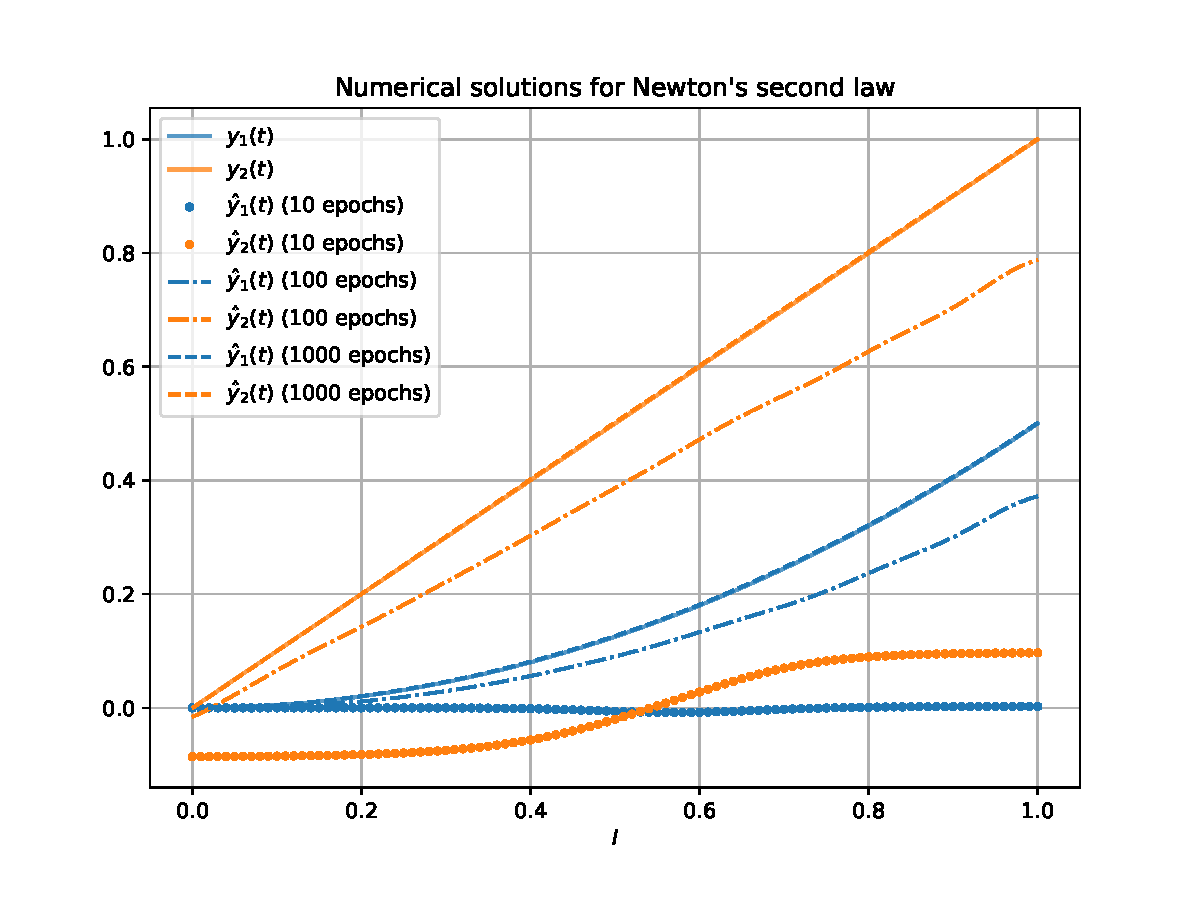
\includegraphics[width=0.8\textwidth]{images/pinn_newton.pdf}
    \caption{Performance of a PINN in comparison to \gls{RK4} in solving an \gls{IVP} of Newton's second law for $I=\left[ 0,1 \right] $. In the graphic, $y_1$ and $y_2$ are the results of the numerical solver, while $\hat{y}_1$ and $\hat{y}_2$ are the results of the PINN trained after different number of epochs.}
    \label{fig:images-pinn_newton-pdf}
\end{figure}


% ---

% ---
% 5 - DEQ
% ---
% ----------------------------------------------------------
\chapter{Deep Equilibrium Models}\label{ch:deq}
% ----------------------------------------------------------

This chapter is dedicated to lay out the foundations of the model architecture that is the central investigation point of this work.
\gls{DEQ}s have been proposed by \textcite{Bai2019} and \textcite{Ghaoui2019}, the latter naming them \emph{implicit models}.
In this chapter, we follow the notation of the former.

Furthermore, one of the greatest challenges in working with \gls{DEQ}s is that, by their implicit nature, they do not fit perfectly well with current deep learning tools.
Therefore, to better understand the nuances and challenges that this family of models present during the experiments, a good share of attention is dedicated to the specificities of performing back propagation with \gls{DEQ}s.

\section{Introduction and Definition}

In Chapter \ref{ch:deep-learning}, the intuition behind a deep learning model was introduced, that is, to model complex features through the composition of simple-yet-non-linear parametrized functions.
Besides the network defined in \ref{sec:neural-nets} (which is the base for \gls{PINN}s, as shown in chapter \ref{ch:pinn}), many other deep learning model architectures have been proposed over the years.
    Some of the architectures with the most surprising results involve composing the models with the same function applied multiple times, i.e., following the notation of chapter \ref{ch:deep-learning}, instead of defining the model as $f_{\gls{param}}=f_{\gls{param}}^{[L]}\circ \cdots \circ f_{\gls{param}}^{[1]}$, these architectures suggest a model similar to $f_{\gls{param}}=f_{\gls{param}}^{[1]}\circ \cdots \circ f_{\gls{param}}^{[1]}$.
Inspired by this, \textcite{Bai2019} takes a step further, defining the model with a (possibly) infinite stack of the same function, which was named \gls{DEQ}.

Let us recall the definition of a deep learning model as proposed in equation \eqref{eq:dl-model}, but imagine it has an infinite number of layers (infinite depth).
Of course, if each $f^{[i]}$ is a different function (with different parameters), then this would be impossible to fit in memory.
Therefore, let us assume that $f_{\gls{param}}^{[i]}=f_{\gls{param}}^{[EQ]},\forall i$, i.e.,
\begin{equation*}
\begin{split}
    z^{[0]} &= x \\
    z^{[i]} &= f_{\gls{param}}^{[EQ]}(z^{[i-1]}), \forall i\ge 1
,\end{split}
\end{equation*}
in which the output would be $z^{\star} = z^{[\infty]}$.
If this iterative process converges, that is, if there is a number $N$ such that $\forall i\ge N,\,z^{[i]}\approx z^{[i+1]}$, then the output $z^{\star}\approx z^{[N]}$ is well-defined, and it is true that  \[
    z^{\star} = f_{\gls{param}}\left( z^{\star} \right) 
.\] 
One can say that $z^{\star}$ is an \emph{equilibrium point} of $f_{\gls{param}}^{[EQ]}$.
Therefore, the output of a well-behaved (i.e., one that respects the restrictions above presented) infinite-depth deep learning model can be computed by finding its equilibrium point.

The model proposed by \textcite{Bai2019} has a slight change in how it handles the input, feeding the input vector at each layer of the model. More precisely, we can say that a \gls{DEQ} of the form
\begin{align*}
    \bm{f}_{\gls{param}}: \R^{n} &\longrightarrow \R^{m} \\
    \bm{x} &\longmapsto \bm{f}_{\gls{param}}(\bm{x}) = \bm{z}^{\star}
\end{align*}
defines its output as the equilibrium point of a function $\bm{f}_{\gls{param}}^{[EQ]}:\R^{n+m}\to \R^{m}$
\begin{equation}\label{eq:z-star}
    \bm{z}^{\star} = \bm{f}_{\gls{param}}^{[EQ]}\left( \bm{x},\bm{z} \right) 
.\end{equation}

\section{Forward}

- naïve approach: iterate the model until an equilibrium is found
- better approach, use any black-box root-finding method
- brief explanation on how root finding methods work? or maybe just introduce quasi-newton methods? or maybe nothing at all?

\subsection{Jacobian Regularization}

- show that a small jacobian => faster convergence

\section{Backward}

\section{Implementation}


% ---

% ---
% 6 - Experiments and Results
% ---
% ----------------------------------------------------------
\chapter{Experiments and Results}\label{ch:experiments}
% ----------------------------------------------------------

In this chapter, we build on the theoretical foundations exposed above and propose a novel solution method for \glspl{IVP} of \glspl{ODE}.
The main goal of the chapter is to validate the approach and explore its performance under different hyperparameter configurations.
This is done through a series of experiments on the Van der Pol oscillator.

We benchmark our approach to \glspl{PINN}, a well-established approach for this kind of problems using deep learning.
The comparison is made both in terms of approximation error and in solution speed.
Overall, this chapter lays out the groundwork for the analysis provided in Chapter \ref{ch:conclusion}.

\section{Problem Definition}

The Van der Pol oscillator (Sec. \ref{sec:vdp}) was chosen as the \gls{ODE} system for which an \gls{IVP} will be solved.
This system is known for having no analytical solution, thus becoming a benchmark for solvers.
As well, \textcite{Antonelo2021} have already studied a solution using \gls{PINN}s, which is considered as a starting point and a reference for performance in the experiments.

More specifically, we define the first-order formulation of the Van der Pol oscillator (as presented in Equation \eqref{eq:vdp}) as the \gls{ODE} system, with $\mu=1$.
Then, the \gls{IVP} is defined with initial condition $\bm{y}(0) = \bm{y}_0 = \left( 0, 0.1 \right) $, simulating a small perturbation to the system around the unstable equilibrium at the origin, and the solution is desired for a horizon of 2 seconds. 
This way, the resulting solution is expected to gravitate to a limit cycle, but not within the solution interval, as illustrated in Figure \ref{fig:vdp_example}.

\subsection{Evaluation Metrics}

As there is no analytical solution to the \gls{IVP} at hand, the solutions will be evaluated in comparison to the approximation found using \gls{RK4}.
This reference was generated from 1000 points equally spaced in the solution interval $I=[0,2]$, with a time step of 2\,ms\footnotemark.
\footnotetext{Of course, this set does not include the initial condition, which is already given, meaning that the first point of evaluation is at $t=0.002$.}
Then, a solution's approximation to the reference is measured through the \gls{IAE}, which can be defined here as \[
    IAE = \frac{1}{h}\sum_{i=1}^{1000} \|\bm{y}_i - \hat{\bm{y}}_i\|
,\] where $\bm{y}_i$ are the points in the \gls{RK4} solution,  $\hat{\bm{y}}_i$ are the points in the solution being evaluated, and $h=0.002$ is the time step.
Therefore, a solution is said to be suitable for the problem if it achieves a low \gls{IAE}.

Besides the quality of the approximation, the time required to achieve such an approximation is also of interest, as many applications (e.g., model predictive control) are highly time-dependent.
As well, the hardware resources used are valuable metrics, as the computing power necessary limits the range of equipment that can support a given solution.
These will be auxiliary to the \gls{IAE} in the analysis of the approximations.

\section{PIDEQ}\label{sec:pideq}

As already discussed in Section \ref{sec:pinn-problem}, solving \gls{IVP}s is (mostly) only reasonable if using a physics-informed approach, that is, if ``teaching'' the model through the known dynamics instead of through actual samples of the target function.
Therefore, a reasonable solution using \gls{DEQ}s must follow the same principle, which implies in a physics-informed training of \gls{DEQ}s (thus, \gls{PIDEQ}).

For the \gls{IVP} defined above, we recall the definition of Section \ref{sec:deq-definition} and propose a \gls{DEQ} similar to \textcite{Ghaoui2019}, that is, a model
\begin{align*}
    D_{\gls{param}}^{EQ}: \R &\longrightarrow \R^2 \\
    t &\longmapsto D_{\gls{param}}(t) = \hat{\bm{y}}
\end{align*}
such that
\begin{equation}
\begin{split}
    D^{EQ}_{\gls{param}}(t) &= C\bm{z}^{\star} \\
    \bm{z}^{\star} &= \bm{f}_{\gls{param}}\left( t,\bm{z}^{\star} \right) \\
    \bm{f}_{\gls{param}}\left( t,\bm{z} \right) &= \tanh \left( A\bm{z} + t\bm{a} + \bm{b} \right)
\end{split}
,\end{equation}
in which the parameters \gls{param} are a vectorization of the matrices and vectors, i.e., $\gls{param} = \left( A,C,\bm{a},\bm{b} \right)$, and the hyperbolic tangent function is applied to each element of the resulting vector.

Notice that this formulation is very close to the one used in Chapter \ref{ch:deq}, except for the linear transformation of the equilibrium point at the model's output.
This implies that both forward and backward operations can occur in the same way, except that the term  \[
    \frac{d D^{EQ}_{\gls{param}}}{d \bm{z}^{\star}} = C
\] must be multiplied in the computation of the gradients.
The advantage of this modification is that we can have $\bm{z}$ with an arbitrary dimension, that is, we can have an arbitrary \emph{number of states}, which results in arbitrary representational power \cite{Ghaoui2019}.

The challenge in physics-informing a \gls{DEQ} is to optimize a cost function on its derivatives.
As it was shown in Section \ref{sec:deq-backward}, \textcite{Bai2019} have proposed an efficient way to compute the first derivative of a \gls{DEQ} with regard to either its parameters or the input, which allows us to compute the cost function value.
Yet, for an application of gradient descent with such cost function, it is required that the second derivatives of the model (with respect to the input and the parameters) are computable during training time.
In practice, this implies in the computation of the derivative of the root-finding algorithm used to compute the first derivative, as seen in Section \ref{sec:deq-backward-implementation}.\footnotemark
\footnotetext{In theory, it could be possible to use the implicit function theorem once again to achieve an analytical formula for the second derivative, but this is left for future work.}
This restricts us to using differentiable root-finding algorithms to compute the first derivative, relying on automatic differentiation tools to compute the second derivative.

Finally, we propose to use a cost function for training a \gls{PIDEQ} model of the form \[
    J\left( \gls{param} \right) = J_b\left( \gls{param} \right) + \lambda J_{\mathcal{N}}\left( \gls{param} \right) + \kappa \left\lVert \frac{d \bm{f}_{\gls{param}}}{d \bm{z}}\right\rVert_F
,\] 
in which $J_b$, $J_{\mathcal{N}}$ and $\lambda$ are as defined in section \ref{sec:PI}, while $\left\lVert \frac{d \bm{f}_{\gls{param}}}{d \bm{z}}\right\rVert_F$ is the Frobenius norm of the Jacobian of the equilibrium function, as exposed in Sec. \ref{sec:deq-jac-reg}, a regularization term weighted by $\kappa \in \R_+$.
This cost function ensures the physics-informed training from \gls{PINN}s with the regularization term which was shown essential to \gls{DEQ}s.

\section{Training}

Early experiments helped to define the design choices for the training algorithm and the hyperparameters.
Adam~\cite{kingma_adam_2015} was the optimizer of choice, with $\gls{lr}=0.001$ and default configuration.
The cost weighting coefficients were initially set as $\lambda=0.1$ and $\kappa=1.0$.
The solver used for the forward pass of the model was the Anderson Acceleration~\cite{walker_anderson_2011}, while best results were found using simple iteration to compute the backward pass.
% \footnotetext{More complex solvers, even if made differentiable for the automatic differentiability package, had such an increased cost for computing the second derivative that the simple iteration became a much better choice.}
For both algorithms, the tolerance was set as $\varepsilon=10^{-4}$ and they were limited to 200 iterations.
The initial guess was always $\bm{z}_0=\bm{0}$.

In regards to the data, $X_b$, of course, contained only the initial condition, while $X_{\mathcal{N}}$ contained $10^5$ random samples within $I$.
The regularization term $\left\lVert \frac{d \bm{f}_{\gls{param}}}{d \bm{z}}\right\rVert_F$ was computed on the input values of both data sets.

\section{Experiments}

The experiments reported below concern the training of the deep learning model proposed above to solve the \gls{IVP} described in the first section of this chapter.
The implementation was done using PyTorch \cite{paszke_pytorch_2019} and is available at \url{https://github.com/brunompacheco/pideq}.
All experiments were performed on a high-end computer, using an RTX 3060 GPU.
A budget of 50000 epochs was chosen.
% TODO add number of runs

\subsection{Baseline Results}

The baseline result for a \gls{PINN} trained to solve an \gls{IVP} of the Van der Pol oscillator comes from \textcite{Antonelo2021}.
We replicate these results, that is, a traditional \gls{PINN} with 4 hidden layers with 20 nodes each, following the same setup proposed above (except for the regularization term of the cost function).
At the same time, \textcite{Ghaoui2019} showed that a \gls{DEQ} with as many states as there are hidden nodes in a given deep feedforward network, has \emph{at least} as much representational power as that network.
Then, our starting \gls{DEQ} is a model with 80 states.
The results for both models can be seen in Figure \ref{fig:baseline-iae}.

\begin{figure}[h]
    \centering
	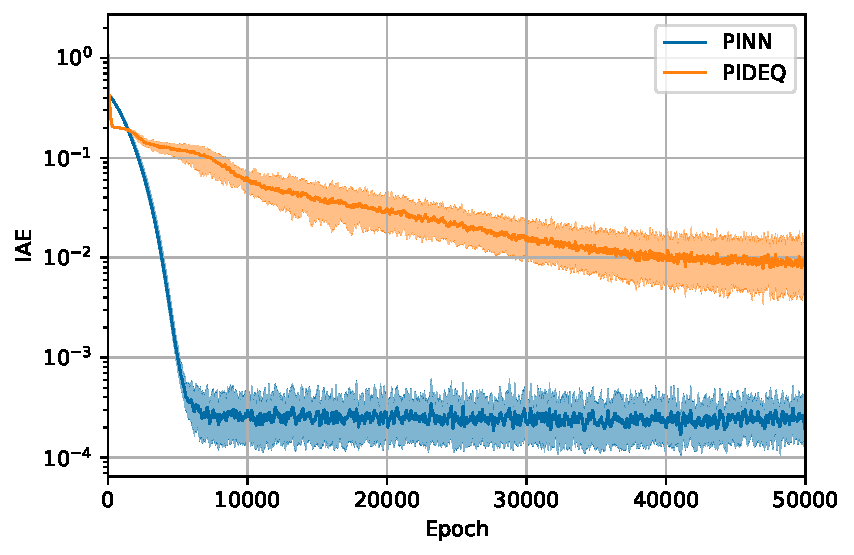
\includegraphics{images/exp_1_iae.pdf}
    \caption{Learning curve for the baseline models trained on the \gls{IVP} for the Van der Pol oscillator. Solid lines are mean values ($n=5$), shaded regions represent minimum and maximum values. For a better visualization, a moving average of 100 epochs was taken.}
    \label{fig:baseline-iae}
\end{figure}

Given that the \gls{PINN} was able to ``learn'' (i.e., to achieve a low IAE on) the task, we expect that the large \gls{PIDEQ} model also is capable of learning.
\glspl{PIDEQ} indeed achieved a low IAE, yet not as low as the \glspl{PINN}.
Furthermore, \glspl{PIDEQ} had a much slower convergence rate, while \glspl{PINN} converged in under 10000 epochs.
Besides being much more complex (in its structure) than the feedforward network, the \gls{PIDEQ} also has many more parameters, in a total of 6802 against 1342.
This results in a big difference in the effective training time: the \gls{PINN}s took, on average, 11\,ms for each epoch, while the \gls{PIDEQ}s took 209\,ms.

\subsection{Number of States}

A deeper look at the $A$ matrix of the baseline \gls{PIDEQ}s after training, as illustrated in Figure \ref{fig:baseline-pideq-A}, shows that many of the rows are practically zero vectors, in comparison to the remaining.
Having ``empty'' rows implies that the states associated with these rows are not effectively contributing to the results, that is, given the parameters of this model, a smaller model could be constructed with the same result.  

\begin{figure}[h]
    \centering
    \begin{subfigure}[t]{.45\textwidth}
	\vspace{0pt}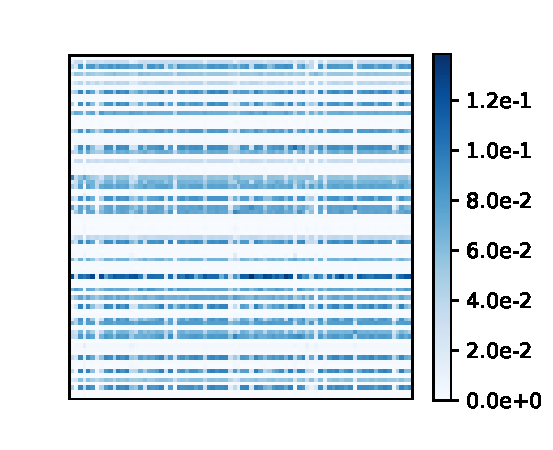
\includegraphics{images/exp_1_matplot.pdf}
	\caption{Magnitude of the elements of $A$. White is 0.}
    \end{subfigure}
    \begin{subfigure}[t]{.45\textwidth}
	\vspace{0pt}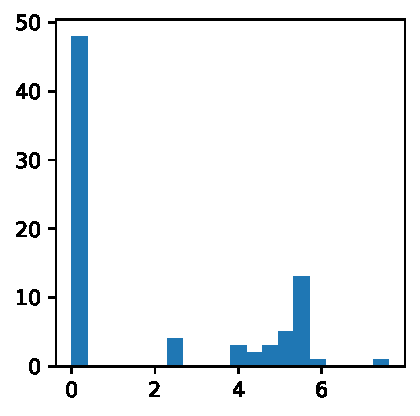
\includegraphics{images/exp_1_hist.pdf}
	\caption{Histogram of $\ell_1$ norm of the rows of $A$.}
    \end{subfigure}
    \caption{$A$ matrix of the baseline \gls{PIDEQ} after training. From all models trained, the one with median final performance was used to generate the graphics.}
    \label{fig:baseline-pideq-A}
\end{figure}

This analysis motivates the training of models with fewer states.
The experiment was defined as an iterative procedure based on the intuition above.
A new model was trained with fewer states, its $A$ matrix was analyzed, and a new model was proposed with even fewer states if there were still empty rows in the $A$ matrix.
This procedure was repeated for models with 40, 20, 10 and 5 states.
The models with 5 states showed no ``empty rows'' in the $A$ matrix, as shown in figure XXX, but still a model with only two states was trained.  % TODO make A matrix figure for #z=5
The results can be seen in Figure \ref{fig:states-iae}.

\begin{figure}[h]
    \centering
    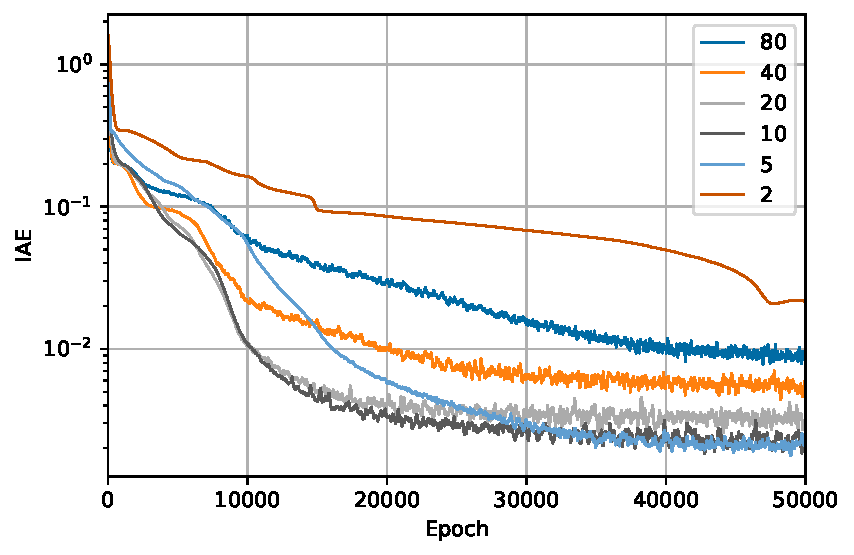
\includegraphics{images/exp_2_iae.pdf}
    \caption{Learning curve of the models trained with fewer states. Solid lines are mean values ($n=5$). For a better visualization, a moving average of 100 epochs was taken.}
    \label{fig:states-iae}
\end{figure}

The smaller models achieve even better results than the baseline and converge much faster, except for the smallest one, which was not able to learn within the training budget, reinforcing the intuition exposed above.
The model with 5 states takes more epochs to converge, intuitively this can be attributed to it being close to its representational limit, but as it is much smaller (with only 52 parameters), it trains faster than the larger ones.
Table \ref{tab:n-states-times} exposes the times for each model.

\begin{table}[h]
    \centering
    \caption{Median training and validation times per epoch for \gls{PIDEQ} models with different number of states.}
    \label{tab:n-states-times}
    \begin{tabular}{ccc}
	\toprule
	\textbf{Number of States} & \textbf{Train} [ms] & \textbf{Validation} [ms] \\ \midrule
	80       & 99.1       & 2.1             \\
	40       & 51.2       & 1.7             \\
	20       & 37.1       & 1.2             \\
	10       & 29.7       & 1.1             \\
	5        & 26.0       & 1.2             \\
	2        & 24.8       & 1.2             \\ \bottomrule
    \end{tabular}
\end{table}

\subsection{Jacobian Regularization}

Following the previous results, the impact of the Jacobian regularization term in the cost function is explored for the model with 5 states.
From the work of \textcite{bai_stabilizing_2021}, it is expected that this regularization term will have an impact on the results.
We verify this by training \gls{PIDEQ} models without such term ($\kappa=0$) and with a reduced importance ($\kappa=0.1$).
The results are shown in Figure \ref{fig:jac-lamb-iae}.

\begin{figure}[h]
    \centering
    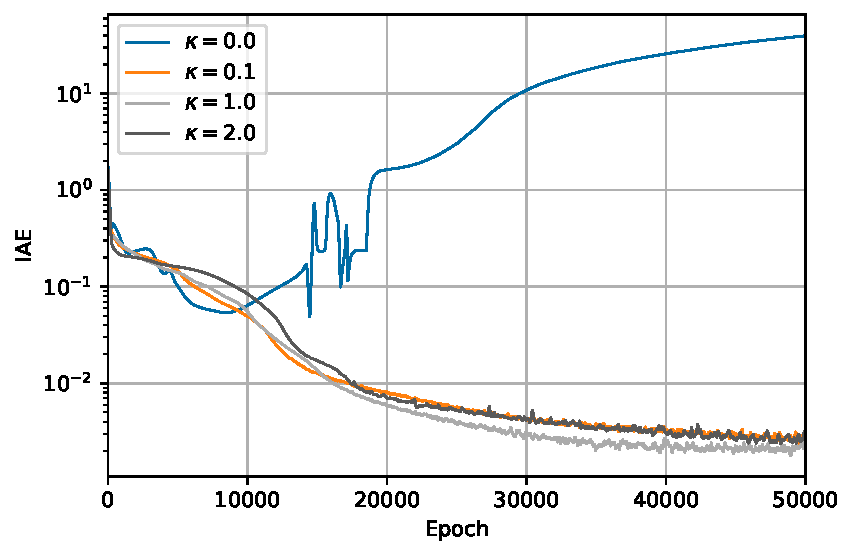
\includegraphics{images/exp_4_iae.pdf}
    \caption{Learning curve for \gls{PIDEQ}s with different $\kappa$ values. Only one model was trained with $\kappa=0$ because the training took over 30 times longer. Solid lines are mean values ($n=5$). For a better visualization, a moving average of 100 epochs was taken.}
    \label{fig:jac-lamb-iae}
\end{figure}

The experiments confirm the theory in that training without the regularization is ineffective.
Not using the regularization term resulted in models not learning the task and taking over 30 times longer to train.
At the same time, increasing or decreasing the impact of the regularization term in the cost function resulted in worse models overall.

\subsection{Solver}

As discussed in Section \ref{sec:pideq}, the solver used within the computation of the first derivative of \glspl{PIDEQ} must be differentiable, and, for the experiments, was fixed as the simple iteration method.
Nevertheless, the impact of the solver used for the forward pass can be explored.
Since the derivative is computed implicitly, solver's impact in the inference and training speed is more clear.
Yet, as the algorithm of different solvers define different paths through the domain to find an equilibrium point, different equilibria can be found given distinct solvers, which can change the performance of the model with respect to error levels. 

In fact, this behavior is observed in the results of the experiments comparing Anderson's Acceleration with simple iteration and Broyden's method~\cite{broyden_class_1965} for the forward pass, as seen in Figure \ref{fig:solver-iae}.
Models using Broyden's method achieve a smaller error, but the iterations took much longer, with a median value of 212 ms in comparison to 27 ms using Anderson Acceleration.
At the same time, using simple iteration resulted in a performance as good as using Anderson Acceleration, but with a median epoch time of 9 ms.
Of course, as was discussed in Section \ref{sec:deq-forward}, simple iteration is less reliable than the other two methods, yet, it seems to work well for the problem at hand.

\begin{figure}[h]
    \centering
    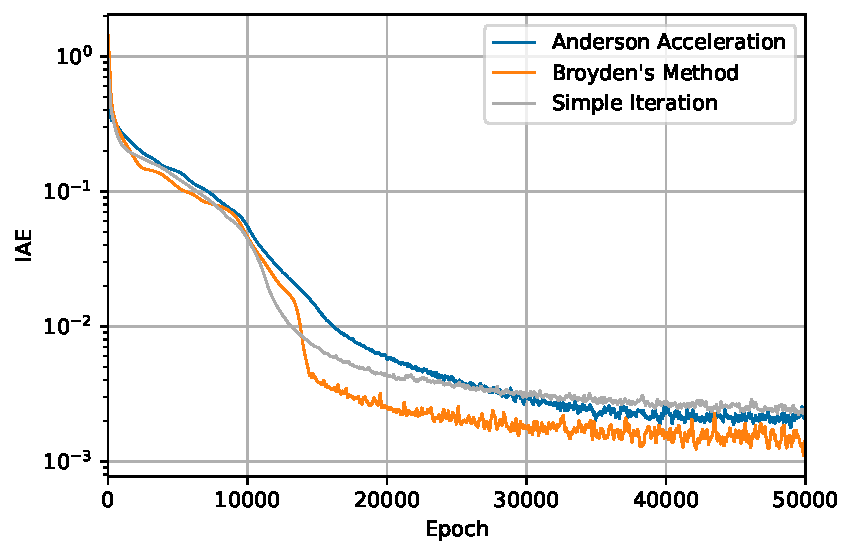
\includegraphics{images/exp_5_iae.pdf}
    \caption{Learning curve of \gls{PIDEQ} models with 5 states using different solvers for the forward pass. Solid lines are mean values ($n=5$). For a better visualization, a moving average of 100 epochs was taken.}
    \label{fig:solver-iae}
\end{figure}

\subsection{Solver Tolerance}

As the previous experiment showed, the simple iteration was the best approach, given the trade-off between prediction quality and training speed.
Then, the $\varepsilon$ parameter is explored next.
Intuitively, it is expected that a smaller tolerance imply in a slower training but a smaller error.
The results with models trained using the simple iteration algorithm with $\varepsilon \in \left[ 10^{-2}, 10^{-4},10^{-6} \right] $, as exposed in figure \ref{fig:epsilon-iae}, confirm that the tolerance is indeed impactful, as increasing the "default" tolerance (of $10^{-4}$) tends to increase the error of the trained models.
At the same time, a decreased tolerance did not provide improve the performance, possibly pointing that the default value is already sufficient for the problem.

\begin{figure}[h]
    \centering
    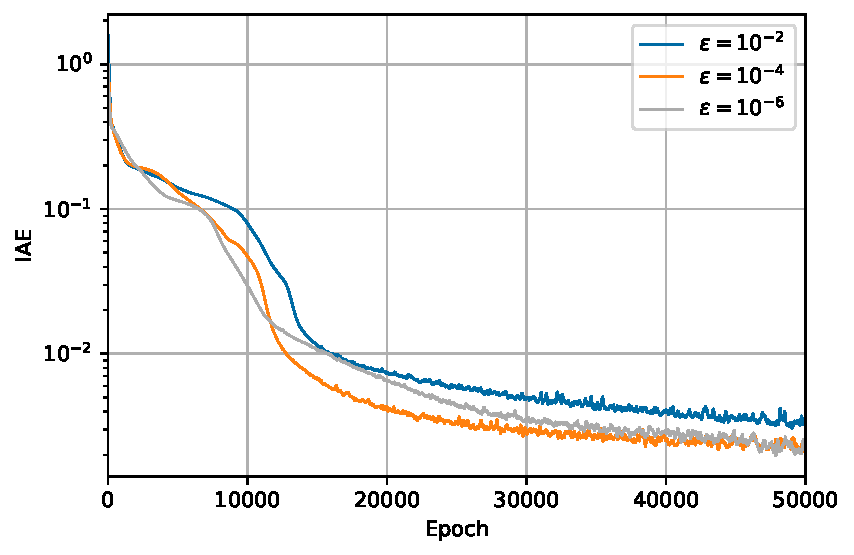
\includegraphics{images/exp_6_iae.pdf}
    \caption{Learning curve of \gls{PIDEQ} models with 5 states when trained with different tolerances for the simple iteration solver. Solid lines are mean values ($n=5$). For a better visualization, a moving average of 100 epochs was taken.}
    \label{fig:epsilon-iae}
\end{figure}

\subsection{Final Model}

The previous experiments showed how much smaller a model can be used and with the simple iteration method, which provides a faster training.
In comparison to the initial \gls{PIDEQ}, there was a significant decrease in the error.
Yet, the biggest impact was in training time, which decreased from 99 ms to 9 ms for each epoch (median value). 
The \gls{PIDEQ} with only 5 states also has significantly fewer parameters (52), since the number of parameters grows quadratically with the number of states.
A reduced number of parameters implies in less memory consumption and in greater explainability.

For a fair comparison, \gls{PINN} models were trained with only 52 parameters, i.e., with only two hidden layers, each with dimension 5.
The performance of the final model and the small \gls{PINN} model can be assessed in Figure \ref{fig:final-iae}, in comparison to the baseline models. The final models can be assessed visually, against \gls{RK4}'s approximate solution, through the graphics in Figure \ref{fig:final-vdp}.

\begin{figure}[h]
    \centering
    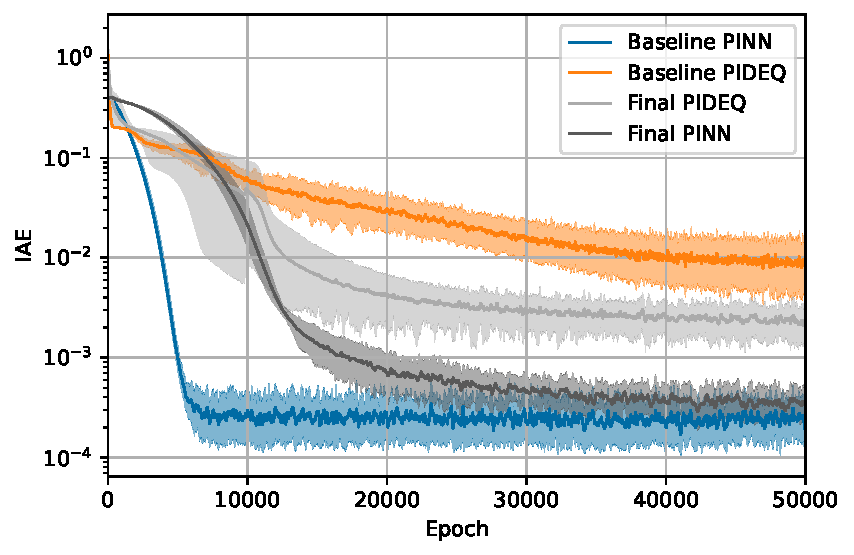
\includegraphics{images/final_iae.pdf}
    \caption{Learning curve of the final models in comparison to the baselines. ``Final PINN'' are the small \gls{PINN} models, with only 52 parameters. ``Final PIDEQ'' are the \gls{PIDEQ} models with 5 states and using the simple iteration method as solver for the forward pass. Solid lines are mean values ($n=5$), shaded regions represent minimum and maximum values. For a better visualization, a moving average of 100 epochs was taken.}
    \label{fig:final-iae}
\end{figure}

\begin{figure}[h]
    \centering
    \begin{subfigure}[t]{.45\textwidth}
	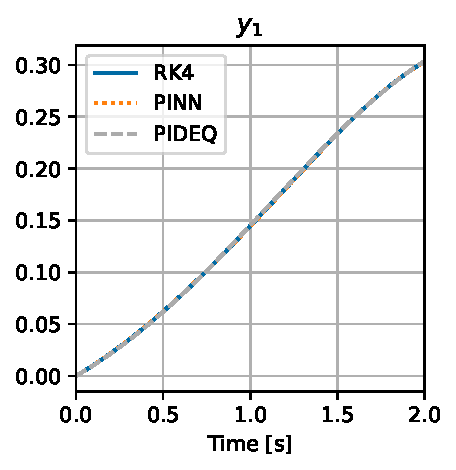
\includegraphics{images/final_vdp_y1.pdf}
	\caption{}
    \end{subfigure}
    \begin{subfigure}[t]{.45\textwidth}
	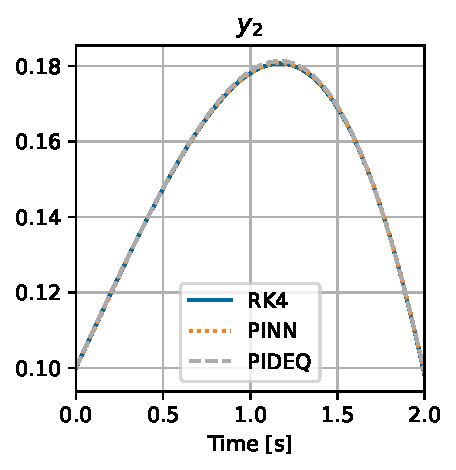
\includegraphics{images/final_vdp_y2.pdf}
	\caption{}
    \end{subfigure}
    \caption{Prediction of \gls{PINN} and \gls{PIDEQ} in comparison to the reference approximation resulting from \gls{RK4}. Both models presented the median performance in the respective experiments.}
    \label{fig:final-vdp}
\end{figure}

Both final models take around the same number of epochs to converge, but the \gls{PINN} models are able to achieve much smaller error, almost as low as the baseline model.
The small \gls{PINN} models, though, have a smaller training time.
A breakdown of the time per epoch spent by each approach can be seen in Figure \ref{fig:final-times}.
It is surprising how the \gls{PIDEQ} models did not take longer than \gls{PINN} models to compute the gradients.
In fact, the biggest impact was on the forward pass, which contributes almost alone to the time difference, overcoming the unexpected efficiency of the cost function computation. 

\begin{figure}[h]
    \centering
    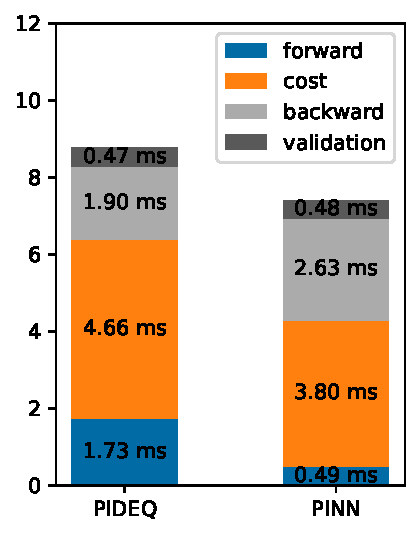
\includegraphics{images/final_times.pdf}
    \caption{Breakdown of median time per epoch for the final \gls{PIDEQ} and the small \gls{PINN}. ``forward'' represents the time necessary to compute the output given the input during the training time (with gradients computation enable). ``cost'' indicates the time necessary to compute the cost function, given the predictions. ``backwards'' is the time necessary to back-propagate the cost to the parameters.}
    \label{fig:final-times}
\end{figure}


% ---

% ---
% 7 - Conclusão
% ---
%\phantompart
% ----------------------------------------------------------
\chapter{Discussion}\label{ch:conclusion}
% ----------------------------------------------------------

- the task is about extracting complex functions out of low-dimensional data, not usual, given the current trends of extracting simpler functions out of high-dimensional data

- We have successfully implemented and trained a physics-informed DEQ model which was able to learn to solve IVPs for the VdP oscillator
- Physics regularization, or any gradient regularization, has never been studied for DEQs
    - they only have first order derivatives well-defined
- the experimental results showed that differentiating through the solver used for computing the first derivative did not have a big impact in the speed of training, computing the equilibrium is still the most costly operation and the biggest difference in comparison to PINN
    - this can be different for larger models, with more complex equilibrium functions, as this would change not only the forward pass but also the Jacobian used by the backward pass

- experimental results with DEQ showed a much slower training and a larger error in comparison to the PINN model, even though both presented very small errors in the proposed problems, to the point of being almost undistinguishable visually
- this points out that the inner structure of DEQ models is not very useful for learning to approximate this type of functions
- we hypothesize that, given DEQ being an approximation to infinite-depth models, it is more suitable to problems that benefit from deeper models
    - however, even a shallow deep feedforward network was able to properly approximate the function




% ----------------------------------------------------------
% ELEMENTOS PÓS-TEXTUAIS
% ----------------------------------------------------------
\postextual
% ----------------------------------------------------------

% ----------------------------------------------------------
% Referências bibliográficas
% ----------------------------------------------------------
\begingroup
    %\printbibliography[title=REFERÊNCIAS]
    \printbibliography
\endgroup

% ----------------------------------------------------------
% Glossário
% ----------------------------------------------------------
%
% Consulte o manual da classe abntex2 para orientações sobre o glossário.
%
%\glossary

% ----------------------------------------------------------
% Apêndices
% ----------------------------------------------------------

% ---
% Inicia os apêndices
% ---
\begin{apendicesenv}
%	\partapendices* 
	% ----------------------------------------------------------
\chapter{Descrição 1}
% ----------------------------------------------------------

Textos elaborados pelo autor, a fim de completar a sua argumentação. Deve ser precedido da palavra APÊNDICE, identificada por letras maiúsculas consecutivas, travessão e pelo respectivo título. Utilizam-se letras maiúsculas dobradas quando esgotadas as letras do alfabeto. 

\end{apendicesenv}
% ---


% ----------------------------------------------------------
% Anexos
% ----------------------------------------------------------

% ---
% Inicia os anexos
% ---
\begin{anexosenv}
%	\partanexos*
	% ----------------------------------------------------------
\chapter{Descrição 2}
% ----------------------------------------------------------

São documentos não elaborados pelo autor que servem como fundamentação (mapas, leis, estatutos). Deve ser precedido da palavra ANEXO, identificada por letras maiúsculas consecutivas, travessão e pelo respectivo título. Utilizam-se letras maiúsculas dobradas quando esgotadas as letras do alfabeto. 

\end{anexosenv}

%---------------------------------------------------------------------
% INDICE REMISSIVO
%---------------------------------------------------------------------
%\phantompart
%\printindex
%---------------------------------------------------------------------

\end{document}
